\documentclass[12pt, a4paper]{report}

% Paquetes esenciales
\usepackage[utf8]{inputenc}
\usepackage[spanish, es-tabla, es-nodecimaldot, es-noshorthands]{babel}
\usepackage[T1]{fontenc}
\usepackage{graphicx}
\usepackage{amsmath, amssymb}
\usepackage{booktabs}
\usepackage{tabularx}
\usepackage{geometry}
\geometry{top=3cm, bottom=3cm, left=3cm, right=3cm}
\usepackage{hyperref}
\usepackage{titlesec}
\usepackage{fancyhdr}
\usepackage{cite}
\usepackage{float}
\usepackage{subcaption}
\usepackage{tikz}
\usepackage{pgfplots}
\pgfplotsset{compat=1.18}
\usepackage{array}
\usepackage{xcolor}
\usetikzlibrary{calc, babel, shapes.geometric, arrows.meta, positioning, fit, backgrounds, shadows}

% Definición de paleta de colores institucional
\definecolor{primary}{RGB}{24, 43, 73}
\definecolor{secondary}{RGB}{70, 130, 180}
\definecolor{lightgray}{RGB}{248, 249, 251}
\definecolor{darkgray}{RGB}{50, 50, 50}
\definecolor{accentblue}{RGB}{2, 136, 209}
\definecolor{accentorange}{RGB}{245, 124, 0}
\definecolor{accentpurple}{RGB}{81, 45, 168}
\definecolor{accentgreen}{RGB}{56, 142, 60}
\definecolor{accentred}{RGB}{198, 40, 40}

% Estilo de títulos
\titleformat{\chapter}{\normalfont\huge\bfseries}{\thechapter.}{20pt}{\Huge}

\title{Integración de Sistema de Visión Artificial y Planificación Dinámica de Trayectorias para una Celda de Clasificación Pick-and-Place sobre una Plataforma Robótica Existente}
\author{Matías Exequiel Molina}
\date{2026}

\begin{document}

\begin{titlepage}
    \centering
    \vspace*{1cm}
    \Large Universidad Nacional de Cuyo \\
    \large Facultad de Ingeniería \\
    \vspace{1cm}
    \Huge \textbf{Proyecto Final de Estudios} \\
    \vspace{0.5cm}
    \large Ingeniería en Mecatrónica \\
    \vspace{2cm}
    \Huge \textbf{Integración de Sistema de Visión Artificial y Planificación Dinámica de Trayectorias} \\
    \vspace{1cm}
    \large \textit{Continuación y evolución del sistema robótico de Agüero y Lezcano} \\
    \vspace{2cm}
    \textbf{Alumno:} Matías Exequiel Molina \\
    \textbf{Director:} Eric Sanchez \\
    \vspace{2cm}
    Mendoza, Argentina \\
    2026
\end{titlepage}

\tableofcontents
\newpage

\chapter{Introducción}
\section{Contexto del Proyecto}
El presente Proyecto Final de Estudios (PFE) constituye una evolución técnica y funcional del manipulador serial de 3 GDL con mecanismo de paralelogramo articulado de cuatro barras para operaciones tipo ``pick-and-place'', desarrollado previamente por Emanuel Agüero y Agustín Lezcano \cite{bib:aguero}. El sistema original ya integraba ROS 2 como estándar de comunicación, una base sólida que este proyecto retoma y potencia para transformar el prototipo en una celda de manufactura más estructurada, escalable y alineada con las buenas prácticas de la ingeniería de software y control embebido.

\section{Evolución, Diagnóstico y Reingeniería del Sistema}
La motivación principal para dar continuidad al proyecto desarrollado por Agüero y Lezcano surgió de la necesidad de evolucionar el prototipo original. El sistema heredado ya integraba clasificación por visión artificial para la manipulación de elementos comerciales, tales como rodamientos, tuercas, tornillos y llaves fijas. Sin embargo, la operación original se limitaba a un enfoque completamente estático, recogiendo las piezas dispuestas directamente sobre una superficie fija de trabajo. El objetivo de este nuevo proyecto fue dar un salto cualitativo hacia el realismo de una celda de manufactura en operación continua, para lo cual se diseñó e incorporó una cinta transportadora física. Esto permitió migrar hacia un sistema dinámico capaz de interceptar los objetos en movimiento basándose íntegramente en la retroalimentación de la visión artificial.

Al recibir la maqueta física y el código fuente, la etapa inicial de relevamiento presentó una alta complejidad técnica, demandando una revisión exhaustiva fundamentada en los conceptos teóricos de robótica y sistemas embebidos de tiempo real \cite{bib:robotica, bib:micro}. El firmware original operaba sobre un archivo monolítico (\texttt{main.c}) con más de 1000 líneas de código. A nivel de software de alto nivel, si bien el nodo de supervisión en ROS 2 era funcional para sus desarrolladores originales, su operación carecía de una interfaz visual orientada al usuario. Debido a la complejidad en la estructura de los comandos y a la curva de aprendizaje inicial del ecosistema ROS 2, durante las primeras pruebas prácticas solo se logró aislar y replicar exitosamente el accionamiento básico del solenoide del efector final. Ante este escenario, y con el propósito de establecer una base sólida, comprensible y escalable para el desarrollo futuro y para futuros alumnos, se decidió realizar una reestructuración profunda.

El primer paso consistió en modularizar el firmware del microcontrolador y desarrollar desde cero una nueva Interfaz Gráfica de Usuario (GUI) interactiva. Esta interfaz se dotó de controles deslizantes para el posicionamiento angular directo de cada motor y comandos discretos para la secuencia de \textit{homing} y la sujeción magnética. El proceso de integración comenzó vinculando la telemetría de los sensores magnéticos de posición hacia la interfaz, lo que permitió observar en tiempo real el comportamiento cinemático al mover el brazo manualmente. Tras verificar esta lectura, se logró la correcta ejecución del \textit{homing} y el solenoide. Posteriormente, se implementó un nuevo tópico dedicado a la recepción de comandos articulares punto a punto (P2P), generando trayectorias con perfiles de velocidad trapezoidal. Esto marcó el primer hito de control autónomo del manipulador.

Sin embargo, durante la fase de validación de movimientos surgieron fallas intermitentes. Los motores Q2 (hombro) y Q3 (muñeca) presentaban vibraciones severas, y en ocasiones, el motor principal de elevación (Q2) perdía la tracción, girando en vacío al recibir una consigna. Para aislar el problema, se procedió a desmontar el brazo y enviar comandos a los motores desacoplados de la estructura, comprobando que el software y la electrónica operaban correctamente. La inspección física reveló dos problemas fundamentales: a nivel eléctrico, un cable de fase del motor Q3 presentaba cortes internos; y a nivel mecánico, existían deficiencias en los acoples de transmisión. Se comprobó que el engranaje impreso del motor Q3 había cedido ante el momento torsor, destruyendo el alojamiento de los prisioneros de fijación, mientras que el motor Q2 había estado operando únicamente por fricción.

Para solucionar esta falla estructural, se llevó a cabo una reingeniería de los acoples. Utilizando un torno y fresas para metal, se mecanizaron los ejes cilíndricos de los motores paso a paso para incorporar un sistema de unión por chaveta. Simultáneamente, se rediseñaron e imprimieron en 3D nuevos engranajes que incluyeran el chavetero, manteniendo la fijación por prisionero original pero trasladando el esfuerzo de torsión a la chaveta. Esta intervención mitigó sustancialmente el deslizamiento y las holguras rotacionales.

Una vez resueltas las fallas de transmisión mecánica, un desafío adicional surgió al integrar el control espacial mediante coordenadas cartesianas (X, Y, Z) en la nueva interfaz. Inicialmente, se empleó el modelo cinemático heredado, el cual utilizaba la convención de Denavit-Hartenberg (D-H) e introducía un eslabón y articulación virtual para modelar matemáticamente la restricción de paralelismo del efector impuesta por el mecanismo de cuatro barras. Sin embargo, la contrastación empírica reveló que esta simplificación no reflejaba con suficiente precisión la pose real del efector final, evidenciando discrepancias sensibles especialmente en la coordenada de altura (Z), la cual resultaba ser la variable más crítica y fácil de medir. Los intentos preliminares de mitigar este error mediante factores de corrección empíricos resultaron insatisfactorios, ya que la calibración convergía solo en regiones acotadas del espacio de trabajo y divergía significativamente en otras.

Tras una revisión de la literatura técnica \cite{bib:kattel}, se decidió descartar el modelo D-H virtualizado y adoptar una aproximación analítica basada en un método geométrico y trigonométrico directo, adaptado específicamente para la morfología de robots con mecanismo de paralelogramo articulado de cuatro barras. La implementación de este nuevo modelo de cinemática en el software resolvió las incongruencias espaciales sistemáticas. Si bien el sistema conserva un error de posicionamiento residual marginal, se determinó que este es atribuible a las tolerancias de fabricación, holguras de rodamientos e imperfecciones elásticas de las piezas impresas en 3D, resultando un desvío admisible para las exigencias de la tarea estipulada.

Finalmente, con la mecánica y la cinemática estabilizadas, se intentó implementar el seguimiento de trayectorias cartesianas continuas. Se configuró la GUI para enviar tramas de posición a intervalos de 10 ms, buscando la velocidad y reacción necesarias para una futura intercepción dinámica de objetos en la cinta. Sin embargo, el movimiento resultante del brazo era errático y presentaba fuertes vibraciones. Un análisis del flujo de datos determinó que la alta tasa de envío generaba un cuello de botella en el canal de comunicación serial entre el orquestador en la PC (ROS 2) y el microcontrolador (micro-ROS y FreeRTOS), provocando latencias y pérdida de paquetes. Como solución arquitectónica para asegurar un perfil de velocidad continuo y determinista, se tomó la decisión de suprimir el cálculo dinámico continuo del planificador en ROS 2 y migrar la totalidad del cálculo analítico de trayectorias al nivel embebido, aprovechando la Unidad de Punto Flotante (FPU) del STM32.

\section{Justificación y Objetivos}
La selección de este PFE se fundamenta en su capacidad para integrar de manera armónica las diversas áreas de la Mecatrónica. La intervención principal se ha centrado en una reingeniería integral: se ha migrado el control hacia una gestión distribuida mediante \textbf{micro-ROS} sobre el \textbf{STM32F446RE}, aplicando principios de código limpio y modular. Asimismo, se optimizó la supervisión mediante una nueva interfaz de control (GUI) intuitiva y se corrigieron deficiencias en la transmisión mecánica y la integridad de señales del bus I2C. Este trabajo reafirma la importancia de la mejora continua sobre plataformas experimentales existentes, consolidando el desarrollo inicial como un banco de ensayos funcional y versátil.

\subsection{Objetivo General}
Desarrollar e integrar el sistema de procesamiento de visión artificial y planificación dinámica de trayectorias para una celda de clasificación industrial a escala, utilizando como base el brazo robótico de 3 GDL existente y una cinta transportadora independiente, logrando la detección, seguimiento y manipulación de objetos en movimiento dentro del periodo operativo estipulado.

\subsection{Objetivos Específicos}
\begin{itemize}
    \item \textbf{Relevamiento y Diagnóstico:} Relevar la arquitectura de control, cinemática y estado actual del sistema robótico existente basándose en el informe técnico de Agüero y Lezcano.
    \item \textbf{Definición de Módulos:} Determinar formalmente qué componentes del firmware y hardware existentes se reutilizan de manera directa y cuáles requieren modificaciones para la nueva aplicación.
    \item \textbf{Procesamiento Digital de Imágenes:} Programar un sistema de visión artificial basado en OpenCV (operando en espacio de color HSV) para segmentar, clasificar objetos en categorías básicas y estimar su posición instantánea (X, Y) sobre la banda de transporte.
    \item \textbf{Desarrollo del Planificador Dinámico:} Diseñar e implementar un algoritmo en el controlador STM32 Nucleo capaz de estimar el punto de intercepción futuro en el espacio de trabajo, sincronizando el efector magnético con la velocidad de la cinta transportadora.
    \item \textbf{Validación del Prototipo:} Evaluar el desempeño global del sistema mediante métricas experimentales de tasa de éxito, repetibilidad y límites operativos de velocidad.
    \item \textbf{Supervisión Remota (Opcional):} Configurar de manera secundaria un nodo de comunicación vía ESP32 para el envío de alertas o visualización de estados en un panel local en Node-RED, supeditado al correcto funcionamiento del lazo principal de pick-and-place.
\end{itemize}

\chapter{Estado del Arte y Antecedentes}
\section{El Proyecto de Agüero y Lezcano}
Este PFE se basa en el desarrollo previo realizado por Agüero y Lezcano, quienes implementaron un manipulador serial de 3 GDL con paralelogramo articulado de cuatro barras con visión artificial utilizando YOLOv11n y comunicación vía ROS 2. Como se observa en la Figura~\ref{fig:pfe_anterior}, su trabajo sentó las bases cinemáticas y la primera aproximación a la visión artificial en la plataforma, proporcionando una estructura impresa en 3D que sirve como chasis funcional.

\begin{figure}[H]
    \centering
    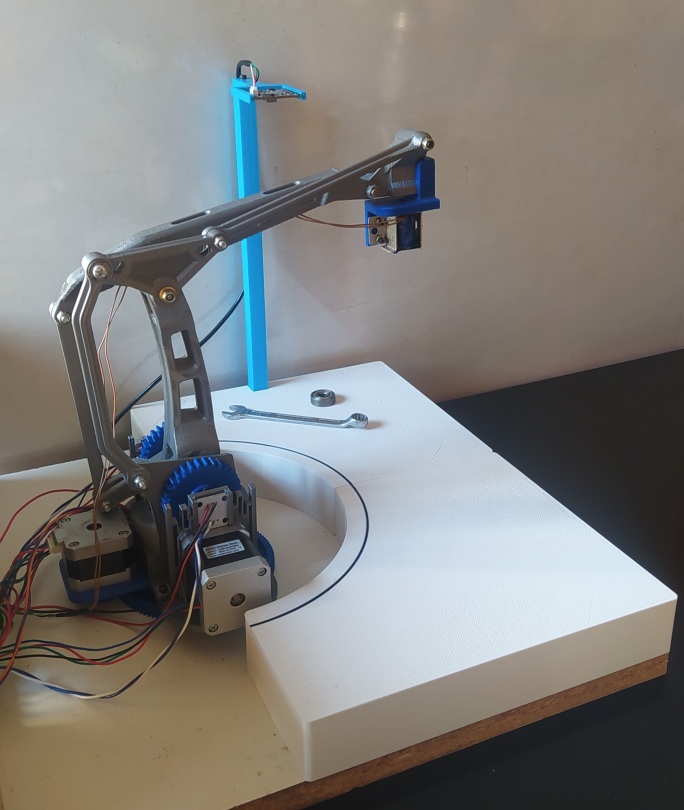
\includegraphics[width=0.7\textwidth]{Imagenes/PFEanterior.png}
    \caption{PFE de Agüero y Lezcano: Manipulador serial de 3 GDL con mecanismo de cuatro barras y visión artificial.}
    \label{fig:pfe_anterior}
\end{figure}

\section{Manipuladores con mecanismo de cuatro barras en impresión 3D}
En el ámbito de la robótica de código abierto, proyectos como \textit{EezyBotArm} han democratizado el acceso a la manipulación robótica (ver Figura~\ref{fig:eezybotarm}). La tendencia actual en la comunidad académica es la migración de actuadores servomotores estándar hacia motores paso a paso con encoders absolutos (como los AS5600 integrados), permitiendo una precisión posicional superior en equipos de laboratorio. La integración de estas mejoras, junto con algoritmos de control de tiempo real, sitúa a este proyecto en el estado del arte de las celdas robotizadas a escala.

\begin{figure}[H]
    \centering
    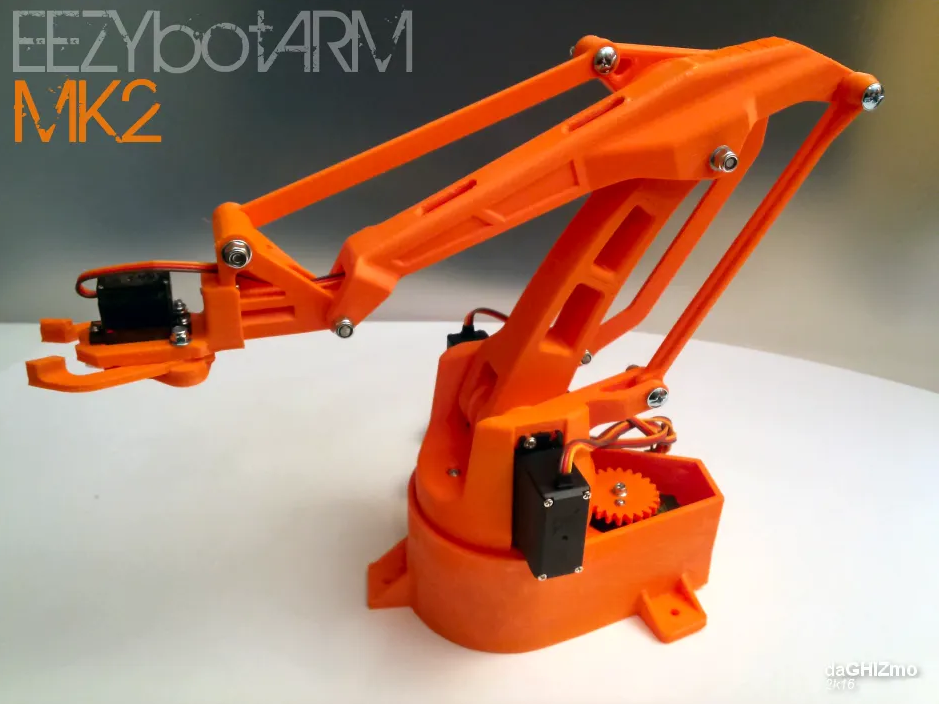
\includegraphics[width=0.7\textwidth]{Imagenes/EezyArmBot.png}
    \caption{Manipulador serial de 3 GDL con mecanismo de paralelogramo de 4 barras.}
    \label{fig:eezybotarm}
\end{figure}

\section{Integración de micro-ROS en Sistemas Embebidos}
La evolución desde ROS 1 hacia ROS 2 ha introducido la capacidad de integrar nodos nativos directamente en microcontroladores mediante micro-ROS. Esta tecnología permite a los microcontroladores (como la familia STM32) participar como entidades de primera clase en el grafo de ROS, garantizando determinismo y reduciendo la latencia de capas intermedias. Su aplicación en sistemas robóticos distribuidos es un pilar fundamental en arquitecturas modernas de manufactura flexible.

\section{Planificación de Trayectorias Dinámicas en Pick-and-Place}
Los sistemas tradicionales de manipulación operan de manera estática: el objeto debe detenerse para ser sujetado. Sin embargo, la industria actual requiere la intercepción dinámica. Los algoritmos modernos combinan la estimación de velocidad del objeto (mediante visión artificial o encoders en las cintas) con la generación de trayectorias polinómicas (ej. quínticas) resueltas en tiempo real, permitiendo sincronizar la velocidad del efector final con la de la cinta transportadora en el momento exacto del agarre.

\begin{figure}[H]
    \centering
    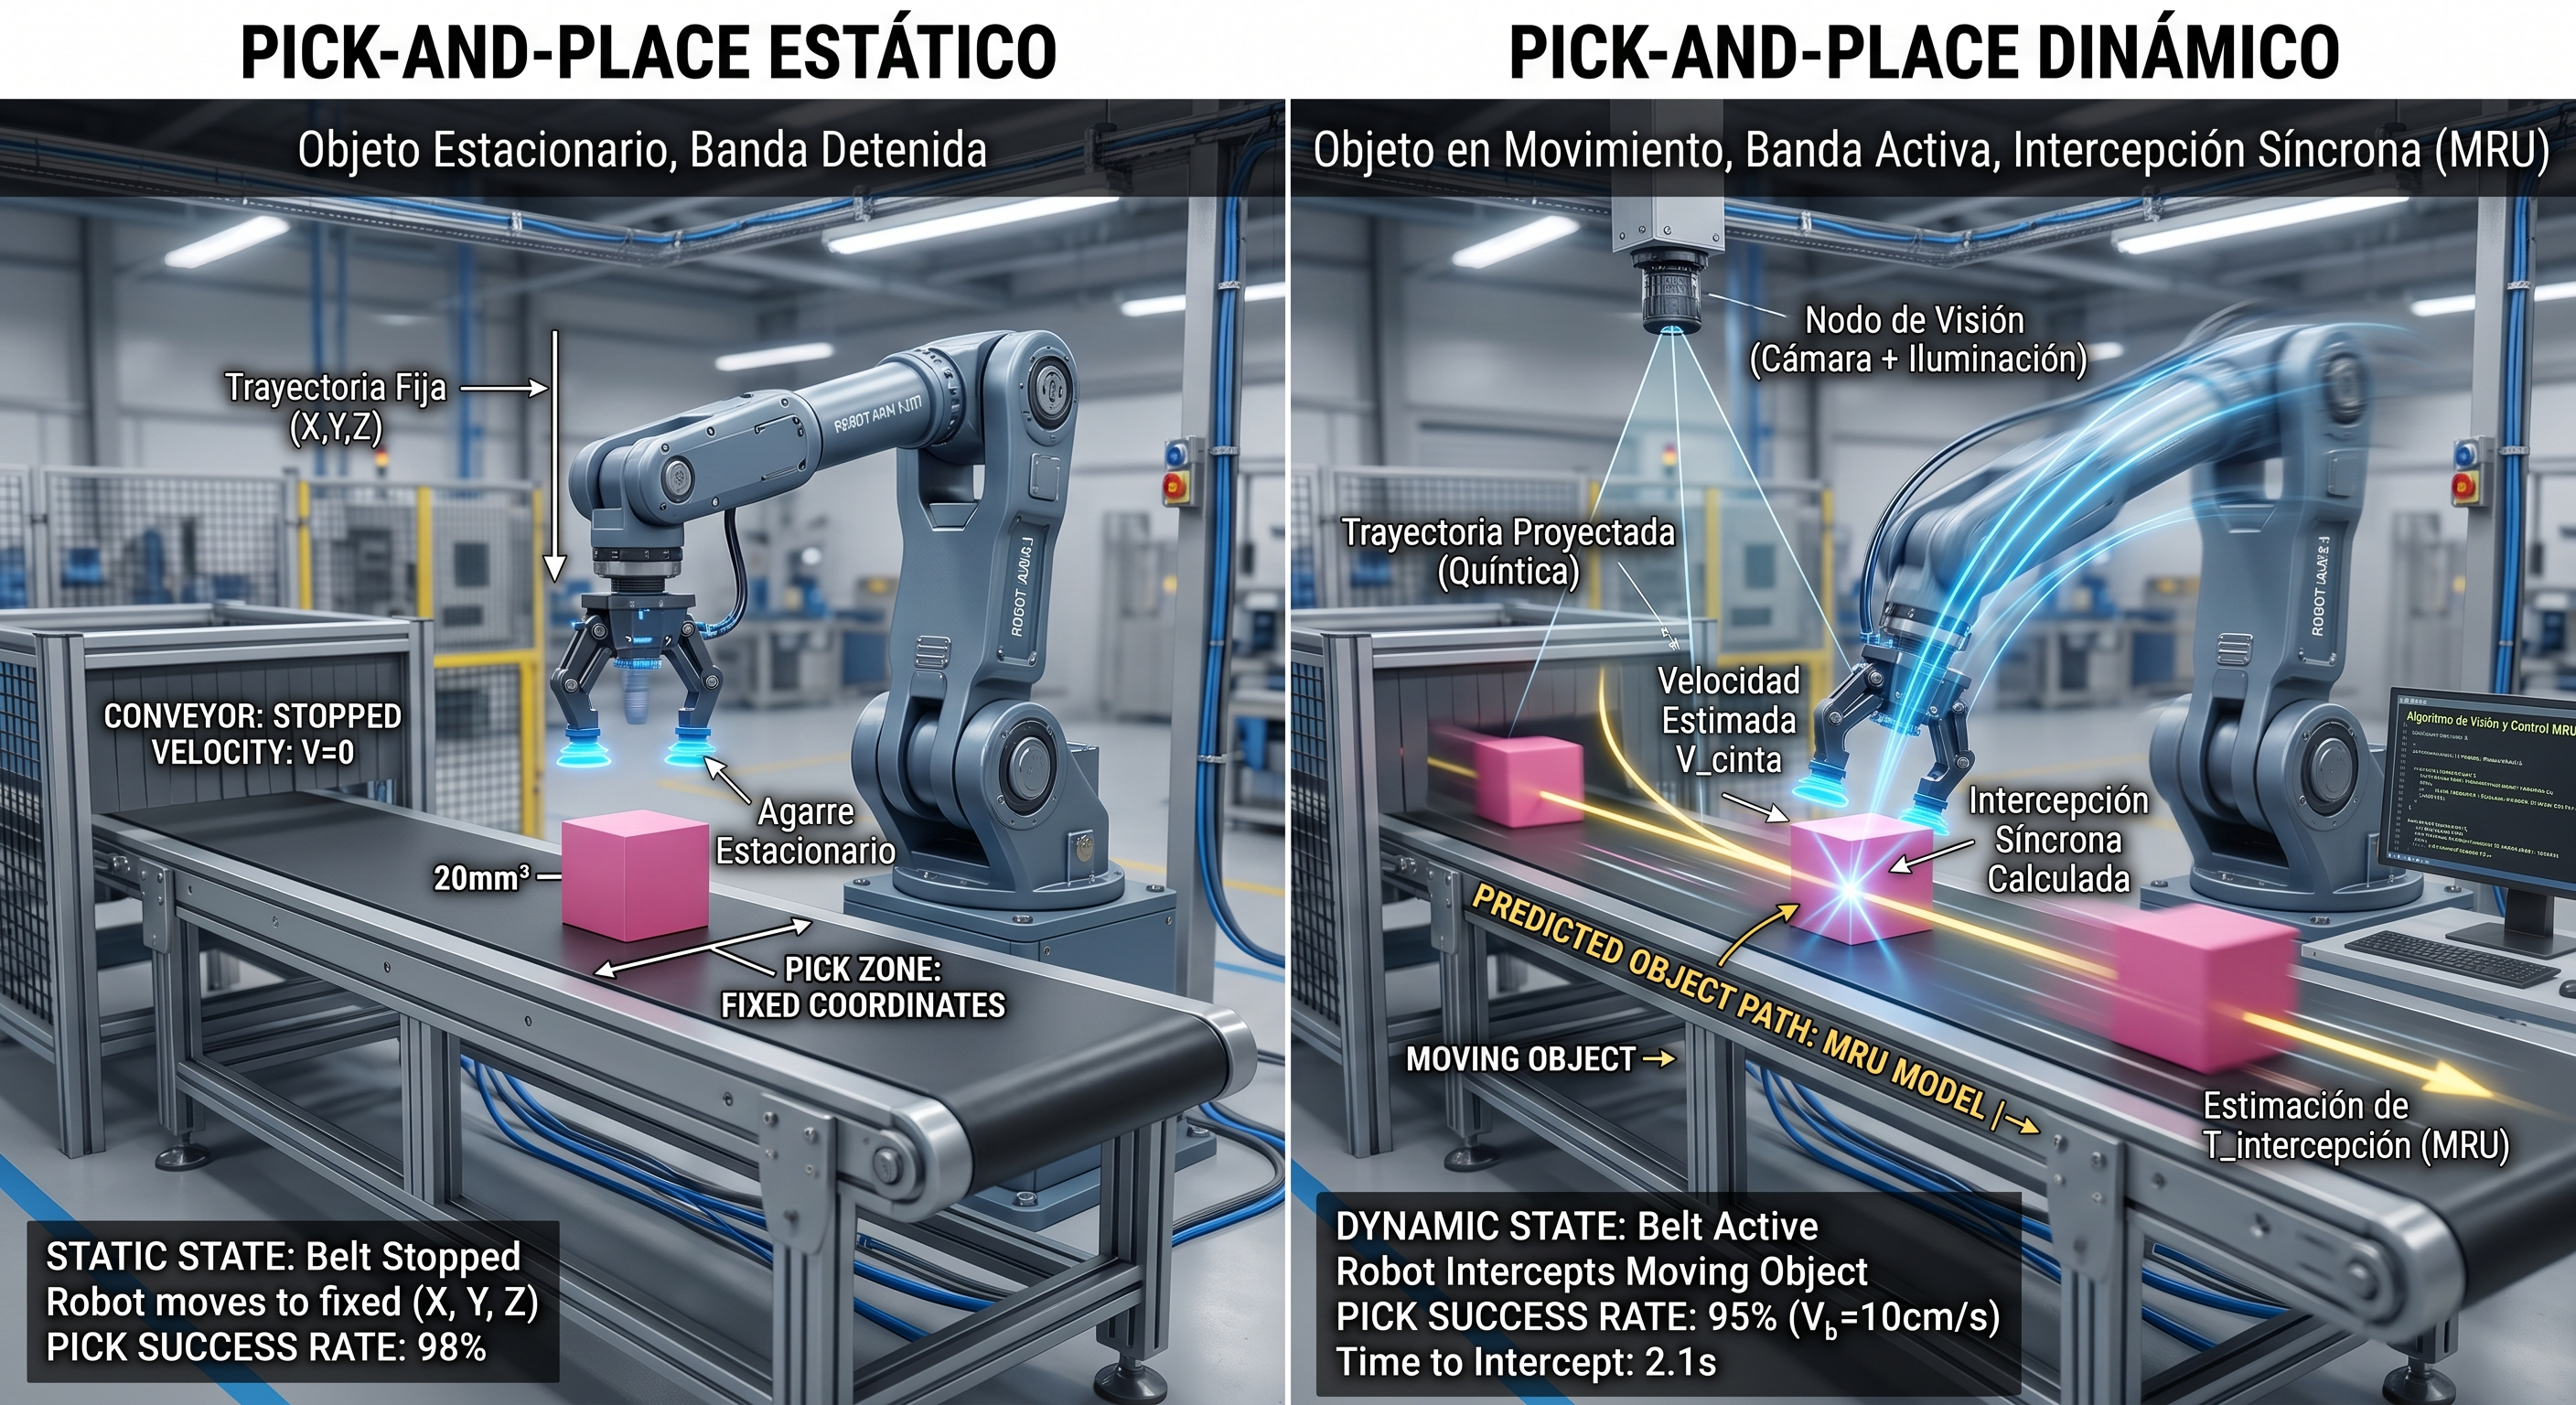
\includegraphics[width=0.95\textwidth]{Imagenes/PickAndPlaceComparacion.jpeg}
    \caption{Comparativa entre Pick-and-Place estático y dinámico.}
    \label{fig:pick_and_place_comparacion}
\end{figure}

\chapter{Arquitectura del Sistema}
\section{Evolución de la Arquitectura de Software y ROS (Antes y Después)}
En el nivel de supervisión y alto nivel (ROS 2), la reingeniería abarcó la totalidad de los nodos de control para asegurar un enlace estructurado y de baja latencia con el microcontrolador:

\begin{itemize}
    \item \textbf{Nodo de Visión Artificial:} Mientras que la versión previa dependía de esquemas fragmentados, en este trabajo se desarrolló un nodo de visión propio y modular basado en sockets asíncronos (\texttt{VisionClient} y \texttt{VisionClientNode}), lo que permite una captura y conversión continua de coordenadas métricas de los objetos detectados.
    \item \textbf{Supresión del Planificador Continuo en ROS:} El nodo planificador continuo que anteriormente operaba en el espacio de ROS 2 fue suprimido de la computadora para las fases dinámicas, reubicando la generación analítica de la curva quíntica directamente en el firmware del STM32. Esto redujo drásticamente el tráfico serial y evitó las discontinuidades en los perfiles de velocidad.
    \item \textbf{Interfaz de Usuario (GUI):} La interfaz original presentaba restricciones operativas. Se programó un módulo gráfico interactivo completamente desde cero (\texttt{RobotUINode} y vistas en PyQt5) dotado de validación de límites articulares y cartesianos, comandos de homing, cinemática inversa y gestión centralizada de la parada por software (\texttt{E-Stop}).
    \item \textbf{Orquestador Central (\texttt{MinimalPublisher} / \texttt{publisher.py}):} El núcleo de coordinación fue modificado para actuar como compuerta de arbitraje y puente de hardware. Administra la máquina de estados del manipulador (\texttt{RobotState}) y la sincronización automática de secuencias operativas multi-segmento ($H \rightarrow A \rightarrow B \rightarrow H$) en conjunto con el servidor de visión.
\end{itemize}

En la Tabla~\ref{tab:comparativa_firmware} se resume la evolución de las características principales de la arquitectura del sistema.

\begin{table}[H]
\centering
\begin{tabular}{p{4cm} p{5cm} p{5cm}}
\toprule
\textbf{Dimensión} & \textbf{Versión Anterior} & \textbf{Versión Actual} \\
\midrule
Organización & Monolítica (\texttt{main.c}) & Modular por componentes \\
Trayectorias & Procesadas en PC & Planificadas en FPU del STM32 \\
Control & Acoplado a ROS & Distribuido (Tareas FreeRTOS) \\
\bottomrule
\end{tabular}
\caption{Comparativa técnica del firmware.}
\label{tab:comparativa_firmware}
\end{table}

La migración hacia una arquitectura distribuida permitió la separación de los subsistemas en módulos independientes (\textit{kinematics}, \textit{trajectory\_planner}, \textit{microros\_callbacks}), facilitando el mantenimiento y la escalabilidad del sistema.

\section{Arquitectura Interna y Flujo de Datos}
La arquitectura de control y comunicación de la celda de manufactura se estructuró en tres niveles de abstracción: el nivel de supervisión y toma de decisiones en la PC host (ROS~2), el puente de comunicaciones de baja latencia (micro-ROS) y el nivel determinista de control embebido en tiempo real. Esta separación garantiza la regularidad en la inyección de señales físicas, un ancho de banda estable para la telemetría y un procesamiento computacional intensivo desacoplado del control directo del hardware.

El subsistema embebido implementado sobre la placa NUCLEO-F446RE desacopla la recepción asíncrona de comandos de alto nivel (vía micro-ROS sobre UART DMA) de la generación determinista de perfiles quínticos y el lazo de control articular ejecutado a 100~Hz bajo FreeRTOS. En la Figura~\ref{fig:mapa_conceptual_firmware} se describe el mapa conceptual global de interacción y acoplamiento funcional entre estos módulos.

\begin{figure}[H]
\centering
\begin{tikzpicture}[
    scale=0.86,
    transform shape,
    auto,
    >=Stealth,
    block/.style={rectangle, draw=black!80, fill=white, thick, text width=4.3cm, align=center, rounded corners=3pt, minimum height=1.15cm},
    hwblock/.style={rectangle, draw=teal!80!black, fill=teal!8, thick, text width=4.1cm, align=center, rounded corners=3pt, minimum height=1.15cm},
    rtosblock/.style={rectangle, draw=orange!80!black, fill=orange!10, thick, text width=4.3cm, align=center, rounded corners=3pt, minimum height=1.15cm},
    mathblock/.style={rectangle, draw=violet!80!black, fill=violet!10, thick, text width=4.1cm, align=center, rounded corners=3pt, minimum height=1.15cm},
    line/.style={draw=black!80, thick, -Latex},
    dashedline/.style={draw=blue!75!black, thick, dashed, -Latex},
    lbl/.style={fill=white, inner sep=2pt, font=\scriptsize, text=black!85, align=center}
]

    % Tronco central
    \node [block] (ros) {
        \textbf{ROS 2 / Supervisión (PC)}\\
        \scriptsize \texttt{/microROS/cmd} \quad \texttt{/planner/traj\_status}
    };
    
    \node [rtosblock, below=1.2cm of ros] (defaulttask) {
        \textbf{\texttt{tasks.c} (\texttt{defaultTask})}\\
        \scriptsize micro-ROS Executor + UART DMA
    };
    
    \node [rtosblock, below=1.3cm of defaulttask] (controltask) {
        \textbf{\texttt{tasks.c} (\texttt{mControlTask})}\\
        \scriptsize Lazo determinista a 100 Hz (10 ms)
    };

    \node [hwblock, below=1.4cm of controltask] (motors) {
        \textbf{\texttt{motors.c}}\\
        \scriptsize Lazo Feedforward + P\\
        \scriptsize Modulación PWM (TIM2, TIM3, TIM13)
    };

    % Columna derecha
    \node [mathblock, right=1.6cm of controltask] (planner) {
        \textbf{\texttt{trajectory\_planner.c}}\\
        \scriptsize Polinomio Quíntico $C^2$\\
        \scriptsize + Fallback Articular
    };
    
    \node [mathblock, below=1.4cm of planner] (kinematics) {
        \textbf{\texttt{kinematics.c}}\\
        \scriptsize FK analítico\\
        \scriptsize e IK trigonométrica
    };

    % Columna izquierda
    \node [hwblock, left=1.6cm of motors] (sensors) {
        \textbf{\texttt{as5600\_tca9548.c}}\\
        \scriptsize Interrupción TIM7 + MUX I2C\\
        \scriptsize 3x Encoders AS5600 (400 kHz)
    };

    % Conexiones
    \draw [line] (ros) -- node[lbl] {Trama UART DMA} (defaulttask);
    \draw [line] (defaulttask) -- node[lbl] {Cola \texttt{mid\_PositionQueue}} (controltask);
    \draw [line] (controltask) -- node[lbl] {$q_{ref}, \dot{q}_{ref}$} (motors);

    \draw [line] ([yshift=3.5mm]controltask.east) -- node[lbl, above] {Ciclo 10 ms} ([yshift=3.5mm]planner.west);
    \draw [line] ([yshift=-3.5mm]planner.west) -- node[lbl, below] {$q_{cmd}, \dot{q}_{cmd}, \text{status}$} ([yshift=-3.5mm]controltask.east);

    \draw [line] ([xshift=-4mm]planner.south) -- node[lbl, left] {$P(t) \rightarrow \text{IK}$} ([xshift=-4mm]kinematics.north);
    \draw [line] ([xshift=4mm]kinematics.north) -- node[lbl, right] {IK / FK OK} ([xshift=4mm]planner.south);

    \draw [line] (sensors) -- node[lbl] {$q_{real}$} (motors);

    \draw [dashedline, rounded corners=6pt] (sensors.north) 
        -- ++(0, 1.4cm) -| node[lbl, pos=0.35, above] {Telemetría 40 Hz} (defaulttask.west);

    \draw [dashedline, rounded corners=8pt] (controltask.west) 
        -- ++(-2.2cm, 0) |- node[lbl, pos=0.35, above, sloped] {Estado (\texttt{traj\_status})} (ros.west);

\end{tikzpicture}
\caption{Mapa de interacción y acoplamiento funcional de los módulos del firmware.}
\label{fig:mapa_conceptual_firmware}
\end{figure}

\subsection{Nivel de Control Embebido (Firmware)}
Para garantizar la ejecución en tiempo real, el firmware del microcontrolador STM32F446RE fue estructurado sobre el sistema operativo FreeRTOS, configurado con un \textit{tick} base de $1\text{ ms}$ y una asignación de memoria dinámica (Heap) de 46 KB. El núcleo de movimiento del robot opera dentro de una tarea dedicada (\texttt{mControlTask}) con alta prioridad y una frecuencia de actualización periódica de 100 Hz ($10\text{ ms}$).

La delegación de la planificación de trayectorias al nivel embebido requirió el diseño de algoritmos de control que consideraran los límites dinámicos de los motores paso a paso:
\begin{itemize}
    \item \textbf{Desacople de Hardware:} Las señales PWM son generadas por los temporizadores TIM2, TIM3 y TIM13, mitigando fluctuaciones temporales provocadas por tareas de software. La lectura de los sensores absolutos AS5600 se estructuró mediante el temporizador TIM7 y un multiplexor I2C, capturando la posición articular de manera periódica.
    \item \textbf{Planificador en Dos Fases:} El algoritmo genera un perfil polinómico de quinto grado ($C^2$). Se limita la velocidad máxima exigida a los actuadores al $85\%$ de su capacidad física admisible (establecida en $1000\text{ Hz}$). Si la duración demandada exige violar este límite, el firmware recalcula la duración ajustándola a la cota mínima calculada en el microcontrolador ($t_{\text{min\_fw}} \ge 0.60\text{ s}$).
    \item \textbf{Asentamiento Terminal:} Al finalizar la curva quíntica, se aplica un control local ($K_{p\_traj} = 3.5$) con tolerancia angular ($0.45^\circ$). Para evitar demoras provocadas por la inercia o la fricción estática de los eslabones impresos en 3D, se configuró una guarda de tiempo límite (\textit{timeout}) de $0.80\text{ s}$, tras el cual se corta la excitación PWM y se concluye la trayectoria informando el estado a la máquina superior.
\end{itemize}

\textbf{Descripción Técnica de los Diagramas de Firmware:}
\begin{itemize}
    \item \textbf{Bloques Principales (Figura~\ref{fig:diagrama_firmware}):} Ilustra el desacoplo temporal del sistema embebido. La tarea \texttt{defaultTask} gestiona la recepción asíncrona de comandos por micro-ROS y deposita las consignas en \texttt{mid\_PositionQueue}. La tarea de alta prioridad \texttt{mControlTask} corre a 100 Hz, consumiendo la cola para alimentar el lazo de control y la generación de pulsos PWM hacia los drivers A4988, mientras los encoders AS5600 proveen retroalimentación angular periódica.
    \item \textbf{Detalle 1 (Figura~\ref{fig:diagrama_firmware_detalle1}):} Detalla el flujo de interrupciones sobre la UART2 con DMA circular. El ejecutor \texttt{rclc} procesa las suscripciones de trayectoria cartesiana, consignas punto a punto articulares, control del solenoide y parada por software. Un temporizador interno a 40 Hz publica la telemetría articular sin saturar el bus serial.
    \item \textbf{Detalle 2 (Figura~\ref{fig:diagrama_firmware_detalle2}):} Muestra el flujo de cálculo en punto flotante (FPU). Al recibir una meta, se valida la cinemática inversa y se ejecuta un perfil quíntico $C^2$. Si el sistema entra en la fase terminal, transiciona a un lazo proporcional con ganancia $K_{p\_traj} = 3.5$ y una ventana de asentamiento de $0.80\text{ s}$ para absorber la fricción mecánica residual.
    \item \textbf{Detalle 3 (Figura~\ref{fig:diagrama_firmware_detalle3}):} Modela la capa de abstracción de hardware (HAL). Los temporizadores TIM2, TIM3 y TIM13 modulan la frecuencia en hercios para los motores paso a paso. En paralelo, el temporizador TIM7 dispara la máquina de estados no bloqueante por I2C que interroga cíclicamente al multiplexor TCA9548A y a los tres sensores magnéticos AS5600.
\end{itemize}

\begin{figure}[H]
    \centering
    \begin{tikzpicture}[
        font=\sffamily\small,
        >=Stealth,
        line width=0.8pt,
        box/.style={
            draw=black!85,
            fill=white,
            line width=1pt,
            align=center,
            inner sep=8pt,
            minimum width=4.8cm,
            drop shadow={opacity=0.15, shadow xshift=2pt, shadow yshift=-2pt}
        },
        queue/.style={
            cylinder,
            draw=black!85,
            fill=white,
            line width=1pt,
            shape border rotate=90,
            aspect=0.25,
            minimum width=3.4cm,
            minimum height=1.6cm,
            align=center,
            inner sep=2pt,
            drop shadow={opacity=0.15, shadow xshift=2pt, shadow yshift=-2pt}
        },
        lbl/.style={
            fill=black!15,
            text=black!90,
            inner sep=3.5pt,
            font=\sffamily\footnotesize,
            align=center
        }
    ]

        \node[box] (sensors) {Sensores 3x Encoders\\AS5600 y TIM7};
        \node[box, below=1.5cm of sensors] (microRos) {defaultTask micro-ROS};
        \node[queue, below=1.4cm of microRos] (queue) {mid\_PositionQueue};
        \node[box, below=1.5cm of queue] (mControl) {mControlTask Control y\\Cinematica};
        \node[box, below=1.4cm of mControl] (actuators) {Actuadores A4988 y\\Motores};

        \draw[->] (sensors) -- node[lbl] {Telemetria 40 Hz} (microRos);
        \draw[->] (microRos) -- node[lbl] {Encola Consigna Cartesiana} (queue);
        \draw[->] (queue) -- node[lbl] {Consume Datos 100 Hz} (mControl);
        \draw[->] (mControl) -- node[lbl] {Genera Pulsos PWM} (actuators);

        \coordinate (bypass) at ([xshift=1.2cm]sensors.east);

        \draw[->, rounded corners=12pt] 
            ([xshift=0.8cm]sensors.south) 
            -- (bypass |- sensors.south) 
            -- node[lbl, midway] {currentAngle} (bypass |- mControl.north) 
            -- ([xshift=1.0cm]mControl.north);

    \end{tikzpicture}
    \caption{Diagrama de bloques Firmware: Bloques Principales de Alto Nivel.}
    \label{fig:diagrama_firmware}
\end{figure}

\begin{figure}[H]
    \centering
    \begin{tikzpicture}[
        font=\sffamily\footnotesize,
        >=Stealth,
        line width=0.8pt,
        box/.style={
            draw=black!85,
            fill=white,
            line width=0.9pt,
            align=center,
            inner sep=5pt,
            minimum height=1.1cm,
            drop shadow={opacity=0.15, shadow xshift=1.5pt, shadow yshift=-1.5pt}
        },
        queue/.style={
            cylinder,
            draw=black!85,
            fill=white,
            line width=0.9pt,
            shape border rotate=90,
            aspect=0.25,
            minimum width=2.9cm,
            minimum height=1.1cm,
            align=center,
            inner sep=3pt,
            drop shadow={opacity=0.15, shadow xshift=1.5pt, shadow yshift=-1.5pt}
        }
    ]

        \node[box, text width=2.8cm] (uart) {UART2 DMA\\Circular};
        \node[box, text width=2.4cm, right=3.4cm of uart] (timer) {Timer 40 Hz};

        \node[box, text width=4.5cm, below=0.8cm of uart] (executor) {\texttt{rclc\_executor\_spin\_some}};
        \node[box, text width=3.4cm, below=0.8cm of timer] (pub) {Publicador:\\\texttt{/microROS/angles}};

        \draw[<->] (uart) -- (executor);
        \draw[->]  (timer) -- (pub);

        \node[box, text width=3.2cm, below=1.3cm of executor, xshift=-5.25cm] (cbCmd) {\texttt{cmd\_callback}\\Trama Cartesiana};
        \node[box, text width=3.2cm, right=0.3cm of cbCmd] (cbP2p) {\texttt{p2p\_cmd\_callback}\\Joints Directos};
        \node[box, text width=3.2cm, right=0.3cm of cbP2p] (cbEm)  {\texttt{electromagnet\_}\\\texttt{callback}\\GPIO};
        \node[box, text width=3.2cm, right=0.3cm of cbP2p] (cbEstop){\texttt{estop\_callback}\\Parada Emergencia};

        \node[queue, below=0.7cm of cbCmd] (queue) {\texttt{mid\_PositionQueue}};

        \draw[->, rounded corners=8pt] (executor.south) -- ++(0,-0.4) -| (cbCmd.north);
        \draw[->, rounded corners=6pt] (executor.south) -- ++(0,-0.4) -| (cbP2p.north);
        \draw[->, rounded corners=6pt] (executor.south) -- ++(0,-0.4) -| (cbEm.north);
        \draw[->, rounded corners=8pt] (executor.south) -- ++(0,-0.4) -| (cbEstop.north);

        \draw[->] (cbCmd) -- (queue);

    \end{tikzpicture}
    \caption{Diagrama de bloques Firmware Detalle 1: defaultTask y micro-ROS.}
    \label{fig:diagrama_firmware_detalle1}
\end{figure}

\begin{figure}[H]
    \centering
    \begin{tikzpicture}[
        font=\sffamily\footnotesize,
        >=Stealth,
        line width=0.8pt,
        box/.style={
            draw=black!85,
            fill=white,
            line width=0.9pt,
            align=center,
            inner sep=5pt,
            drop shadow={opacity=0.15, shadow xshift=1.5pt, shadow yshift=-1.5pt}
        },
        decision/.style={
            diamond,
            draw=black!85,
            fill=white,
            line width=0.9pt,
            align=center,
            inner sep=3pt,
            aspect=1.4,
            drop shadow={opacity=0.15, shadow xshift=1.5pt, shadow yshift=-1.5pt}
        },
        lbl/.style={
            fill=black!18,
            text=black!90,
            inner sep=2.5pt,
            font=\sffamily\scriptsize,
            align=center
        }
    ]

        \node[box, text width=3.8cm] (init) {Bucle Control\\100 Hz 10 ms};
        \node[decision, text width=2.4cm, below=0.8cm of init] (decCola) {Dato en Cola?};

        \node[box, text width=4.0cm, below right=0.9cm and 0.2cm of decCola] (trajStart) {\texttt{TrajectoryPlanner\_StartCtraj}\\IK + t\_min\_fw};

        \node[decision, text width=2.8cm, below=2.8cm of decCola] (decActiva) {Trayectoria\\Activa?};

        \node[box, text width=3.6cm, below left=1.0cm and 0.4cm of decActiva] (trayQuintica) {Trayectoria Quintica C2 +\\Asentamiento};
        \node[decision, text width=2.2cm, below right=0.9cm and 0.5cm of decActiva] (decP2P) {Modo P2P?};

        \node[box, text width=3.0cm, below=1.0cm of trayQuintica] (ctrlPd) {Lazo Feedforward + P\\Kp=3.5};
        \node[box, text width=2.5cm, below=1.0cm of decP2P] (p2pRamp) {\texttt{updateP2PRamp}};

        \node[box, text width=3.0cm, below=1.0cm of decActiva |- ctrlPd.south] (stepper) {\texttt{Stepper\_SetSpeed}\\Hz};

        \draw[->] (init) -- (decCola);
        \draw[->] (decCola.east) to[out=-30, in=90] node[lbl, pos=0.35] {Si} (trajStart.north);
        \draw[->] (decCola.west) to[out=210, in=150] node[lbl, midway] {No} (decActiva.north west);
        \draw[->] (trajStart.south) to[out=-90, in=30] (decActiva.north east);
        \draw[->] (decActiva.south west) to[out=210, in=90] node[lbl, midway] {Si} (trayQuintica.north);
        \draw[->] (decActiva.south east) to[out=-30, in=90] node[lbl, midway] {No} (decP2P.north);
        \draw[->] (trayQuintica) -- (ctrlPd);
        \draw[->] (decP2P) -- node[lbl, midway] {Si} (p2pRamp);
        \draw[->] (ctrlPd.south)  to[out=-90, in=120] ([xshift=-0.7cm]stepper.north);
        \draw[->] (p2pRamp.south) to[out=-90, in=60]  ([xshift=0.7cm]stepper.north);

    \end{tikzpicture}
    \caption{Diagrama de bloques Firmware Detalle 2: mControlTask y Planificador Quíntico.}
    \label{fig:diagrama_firmware_detalle2}
\end{figure}

\begin{figure}[H]
    \centering
    \begin{tikzpicture}[
        font=\sffamily\footnotesize,
        >=Stealth,
        line width=0.8pt,
        box/.style={
            draw=black!85,
            fill=white,
            line width=0.9pt,
            align=center,
            inner sep=4pt,
            text width=3.8cm,
            minimum height=1.05cm,
            drop shadow={opacity=0.15, shadow xshift=1.5pt, shadow yshift=-1.5pt}
        }
    ]

        \node[box] (c1r1) at (0, 0)       {Frecuencia de Paso Hz};
        \node[box] (c2r1) at (4.6, 0)     {Timer TIM7 IT};
        \node[box] (c3r1) at (9.2, 0)     {Comando Electroiman};

        \node[box] (c1r2) at (0, -1.6)   {TIM13 Q1, TIM2 Q2,\\TIM3 Q3};
        \node[box] (c2r2) at (4.6, -1.6) {Multiplexor I2C\\TCA9548A};
        \node[box] (c3r2) at (9.2, -1.6) {GPIO PC3 MOSFET\\+ PC7 LED};

        \node[box] (c1r3) at (0, -3.2)   {Drivers A4988\\1/8 Micropasos};
        \node[box] (c2r3) at (4.6, -3.2) {3x Sensores AS5600};

        \node[box] (c1r4) at (0, -4.8)   {Motores Paso a Paso\\NEMA};
        \node[box] (c2r4) at (4.6, -4.8) {{\scriptsize\texttt{motor1/2/3.currentAngle}}};

        \draw[->] (c1r1) -- (c1r2);
        \draw[->] (c1r2) -- (c1r3);
        \draw[->] (c1r3) -- (c1r4);

        \draw[->] (c2r1) -- (c2r2);
        \draw[->] (c2r2) -- (c2r3);
        \draw[->] (c2r3) -- (c2r4);

        \draw[->] (c3r1) -- (c3r2);

    \end{tikzpicture}
    \caption{Diagrama de bloques Firmware Detalle 3: Periféricos y Hardware Físico.}
    \label{fig:diagrama_firmware_detalle3}
\end{figure}

\begin{table}[H]
\centering
\small
\begin{tabular}{|p{3.3cm}|p{2.3cm}|p{2.6cm}|p{5.8cm}|}
\hline
\textbf{Parámetro / Macro} & \textbf{Valor} & \textbf{Módulo} & \textbf{Justificación y Criterio} \\
\hline
\texttt{configTOTAL\_}\linebreak\texttt{HEAP\_SIZE} & 46 KB & \texttt{FreeRTOS.h} & Memoria dinámica para stacks de tareas y buffers de micro-ROS. \\
\hline
\texttt{CONTROL\_LOOP\_}\linebreak\texttt{PERIOD} & 100 Hz (10 ms) & \texttt{tasks.c} & Periodo de cómputo del planificador quíntico y control. \\
\hline
\texttt{timer\_period} & 40 Hz (25 ms) & \texttt{tasks.c} & Telemetría angular sin saturar canal UART/DMA. \\
\hline
Bus I2C & 400 kHz & \texttt{main.c} & Muestreo de 3 encoders AS5600 vía TIM7 sin bloqueo. \\
\hline
\texttt{MAX\_V\_HZ} & 1000 Hz & \texttt{motors.h} & Límite a 1/8 micropaso para evitar pérdidas de paso. \\
\hline
\texttt{max\_freq\_safe} & 850 Hz (85\%) & \texttt{traj\_planner.c} & Margen del 15\% para control proporcional sin saturación. \\
\hline
\texttt{t\_min\_fw} & 0.60 s & \texttt{traj\_planner.c} & Cota temporal inferior del generador quíntico embebido. \\
\hline
\texttt{Kp\_traj} & 3.50 & \texttt{motors.c} & Ganancia proporcional de seguimiento y asentamiento. \\
\hline
\texttt{ANGLE\_}\linebreak\texttt{TOLERANCE} & $0.25^\circ$ / $0.45^\circ$ & \texttt{main.h} & Ventana de convergencia para corte de excitación PWM. \\
\hline
Timeout Asentamiento & 0.80 s & \texttt{traj\_planner.c} & Límite temporal para evitar demoras por fricción residual. \\
\hline
\end{tabular}
\caption{Parámetros operativos y criterios de diseño del Firmware (STM32 / FreeRTOS).}
\label{tab:parametros_firmware}
\end{table}

\subsubsection{Estructura del Lazo Articular: Control Feedforward + P}
A diferencia de un esquema PID clásico puro donde la señal depende enteramente de la acumulación histórica del error, el seguimiento dinámico de las trayectorias cartesianas se rige por un esquema de prealimentación de velocidad (\textit{feedforward}) acoplado a una realimentación proporcional (P) de posición \cite{bib:craig}.

\begin{figure}[htbp]
\centering
\begin{tikzpicture}[
    auto,
    block/.style={draw=darkgray, fill=white, thick, rectangle, minimum height=1cm, minimum width=1.5cm, text centered},
    sum/.style={draw=darkgray, fill=white, thick, circle, inner sep=2pt},
    input/.style={coordinate},
    output/.style={coordinate},
    arr/.style={draw=darkgray, thick, -Latex}
]
    \node [input] (qd_in) at (0, 1.5) {};
    \node [input] (q_in) at (0, 0) {};
    
    \node [sum] (sum_err) at (1.6, 0) {$+$};
    \node [block] (kp) at (3.4, 0) {$K_{p\_traj}$};
    
    \node [sum] (sum_ff) at (5.2, 0) {$+$};
    
    \node [block, text width=2.5cm] (robot) at (7.8, 0) {Robot / Driver A4988};
    \node [output] (out) at (10.4, 0) {};
    
    \node [block, text width=2.4cm] (sensor) at (7.8, -1.5) {Encoder AS5600};

    \draw [arr] (qd_in) -- node[above, near start] {$\dot{q}_{ref}(t)$ (Feedforward)} ++(5.2, 0) -- (sum_ff);
    
    \draw [arr] (q_in) -- node[above] {$q_{ref}(t)$} (sum_err);
    \draw [arr] (sum_err) -- node[above] {$e(t)$} (kp);
    \draw [arr] (kp) -- (sum_ff);
    
    \draw [arr] (sum_ff) -- node[above] {$v_{cmd}(t)$} (robot);
    \draw [arr] (robot) -- node[above] {$q(t)$} (out);
    
    \draw [arr] ($(robot.east)!0.5!(out)$) |- (sensor);
    \draw [arr] (sensor) -| node[pos=0.9, left] {$-$} (sum_err);

\end{tikzpicture}
\caption{Diagrama en bloques del lazo de control con prealimentación de velocidad (feedforward) y realimentación proporcional de posición.}
\label{fig:diagrama_control_ff}
\end{figure}

\paragraph{1. Modo Trayectoria Continua Quíntica (\texttt{TRAJ}): Velocidad Feedforward a 100 Hz}
En este modo, la referencia es un \textbf{vector dinámico instantáneo} $\mathbf{\dot{q}_{ref}(t)}$ (\texttt{qd\_ref} en $[^\circ/\text{s}]$) evaluado cada $\Delta t = 10\text{ ms}$ mediante la derivada analítica discreta de las consignas quínticas:
\begin{equation}
    \dot{q}_{ref}[i] = \frac{q_{current}[i] - q_{last}[i]}{\Delta t} \quad [^\circ/\text{s}]
\end{equation}
Esta señal entra directamente como prealimentación (\textit{feedforward}) al lazo implementado en \texttt{motors.c}:
\begin{equation}
    v_{cmd}(t) = \dot{q}_{ref}(t) + K_{p\_traj} \cdot \big(q_{ref}(t) - q_{real}(t)\big) \quad [^\circ/\text{s}]
\end{equation}
donde $K_{p\_traj} = 3.50$. La velocidad resultante se convierte en pulsos de excitación PWM para los controladores (A4988) considerando la reducción mecánica $i$ y la resolución a $1/8$ de micropaso ($1600\text{ pulsos/rev}$, equivalente a $\text{\texttt{DEG\_TO\_STEPS}} = 4.444\dots\text{ pulsos}/^\circ$):
\begin{equation}
    f_{PWM}\text{ [Hz]} = |v_{cmd}| \cdot \left(\frac{1600\text{ pulsos}}{360^\circ}\right) \cdot i
\end{equation}
Cotas de saturación:
\begin{itemize}
    \item \textbf{Corte por Velocidad Mínima:} Si $f_{PWM} < 1.0\text{ Hz}$ (\texttt{TRAJ\_CUTOFF\_FREQ\_HZ}), se desactiva la salida para evitar zumbidos residuales en los bobinados.
    \item \textbf{Límite Dinámico Superior:} $f_{PWM} \le 1000\text{ Hz}$ (\texttt{MAX\_V\_HZ}). El planificador restringe la velocidad pico de la curva al 85\% ($850\text{ Hz}$, \texttt{TRAJ\_MAX\_SAFE\_FREQ\_HZ}) para reservar un 15\% de margen al término proporcional.
\end{itemize}

\paragraph{2. Modo Punto a Punto (\texttt{P2P}): Velocidades de Régimen y Rampas}
En traslados manuales o rutinas de origen (\textit{homing}) gestionadas por temporizadores de hardware:
\begin{itemize}
    \item \textbf{Velocidad Nominal por Defecto:} $\text{\texttt{SPEED\_P2P\_DEFAULT\_HZ}} = 350.0\text{ Hz}$.
    \item \textbf{Velocidad Base de Arranque:} $\text{\texttt{MIN\_SPEED\_HZ}} = 150.0\text{ Hz}$.
    \item \textbf{Sincronización Multieje:} \texttt{startSynchronizedP2PMovement()} calcula la velocidad de régimen $v_{scaled} \in [280, 1000]\text{ Hz}$ para cada eje escalándola al tiempo del motor con mayor desplazamiento angular.
\end{itemize}

\subsubsection{Responsabilidad Específica de los Módulos del Firmware}

\paragraph{\texttt{main.c} --- Configuración del Microcontrolador y Recursos Base}
\begin{itemize}
    \item \textbf{Inicialización del Reloj:} Núcleo STM32F446RE a 180~MHz vía oscilador HSI acoplado al PLL ($M=8$, $N=180$, $P=2$).
    \item \textbf{Mapeo de Temporizadores PWM (Shield A4988):}
    \begin{itemize}
        \item \texttt{TIM13} (CH1) $\rightarrow$ Motor 1 (Cintura / Q1) --- 16 bits (ARR máx: $65535$).
        \item \texttt{TIM2} (CH2) $\rightarrow$ Motor 2 (Hombro / Q2) --- 32 bits (ARR máx: $4294967295$).
        \item \texttt{TIM3} (CH2) $\rightarrow$ Motor 3 (Muñeca / Q3) --- 16 bits (ARR máx: $65535$).
    \end{itemize}
    \item \textbf{Prevención de Overflow en ARR:} Como $\text{ARR} = (f_{timer}/f_{PWM}) - 1$, frecuencias menores a $2\text{ Hz}$ desbordarían registros de 16 bits. \texttt{Stepper\_SetSpeed()} satura a $65535$ y corta el pulso si $f < 2\text{ Hz}$.
    \item \textbf{Recursos FreeRTOS:} Instancia \texttt{mid\_PositionQueue} con capacidad para 4 consignas \texttt{CARTESIAN\_CMD\_t}.
\end{itemize}

\paragraph{\texttt{tasks.c} --- Concurrencia FreeRTOS y Transporte micro-ROS}
\begin{itemize}
    \item \textbf{\texttt{defaultTask} (Prioridad Normal --- Stack 8 KB):}
    Atiende micro-ROS vía UART2 DMA (115200 bps). Encola consignas cartesianas desde \texttt{/microROS/cmd}, procesa la parada por software en \texttt{/microROS/emergency\_stop} y publica ángulos a 40~Hz en \texttt{/microROS/angles}.
    \item \textbf{\texttt{mControlTask} (Alta Prioridad --- 100 Hz, Stack 4 KB):}
    Ejecutada periódicamente cada 10~ms con \texttt{vTaskDelayUntil()}. Desencola consignas de \texttt{mid\_PositionQueue}, evalúa \texttt{TrajectoryPlanner\_Update()}, modula el lazo Feedforward + P hacia \texttt{motors.c} y publica el estado en \texttt{/planner/traj\_status}.
\end{itemize}

\paragraph{\texttt{trajectory\_planner.c} --- Generador Quíntico y Fallback Articular}
Genera perfiles suaves con velocidad y aceleración nulas en extremos:
\begin{equation}
    s(\tau) = 10\tau^3 - 15\tau^4 + 6\tau^5, \quad \tau = \frac{t}{T} \in [0, 1]
\end{equation}
\begin{enumerate}
    \item \textbf{Fase de Arranque (\texttt{StartCtraj}):}
    Valida la cinemática inversa (IK) del destino y registra la pose articular inicial $\mathbf{q_{start}}$. Calcula el tiempo mínimo dinámico local evaluando la derivada pico ($1.875$):
    \begin{equation}
        t_{\text{min\_fw}} = \max\left(0.60\text{ s}, \, \max_{i \in \{1,2,3\}} \frac{1.875 \cdot \Delta q_i \cdot \text{DEG\_TO\_STEPS} \cdot i_{red}[i]}{850\text{ Hz}}\right)
    \end{equation}
    Nótese que este valor representa la cota inferior algorítmica del microcontrolador ante desplazamientos mínimos, diferenciándose de la guarda operativa del supervisor ($T_{\text{MIN\_ROBOT}}$) requerida para el traslado completo desde la guardia hasta la cinta.
    \item \textbf{Fase 1 ($\tau < 1.0$ --- Interpolación Quíntica y Fallback):}
    Interpola $P(t) = P_{start} + s(\tau)(P_{target} - P_{start})$. Si la recta cartesiana atraviesa una singularidad o excede el espacio de trabajo, \texttt{Kinematics\_IK()} falla y el firmware conmuta de forma continua al espacio articular:
    \begin{equation}
        q_{cmd}[i](t) = q_{start}[i] + s(\tau) \cdot \big(q_{target}[i] - q_{start}[i]\big)
    \end{equation}
    garantizando arribo a destino sin discontinuidades bruscas de velocidad ni interrupción del ciclo.
    \item \textbf{Fase 2 ($\tau \ge 1.0$ --- Asentamiento Terminal):}
    Mantiene $q_{target}$ con feedforward nulo. Supervisa que $|q_{target}[i] - q_{real}[i]| \le 0.45^\circ$. Si converge retorna \texttt{SUCCESS} (2); si expiran $0.80\text{ s}$ (\texttt{TRAJ\_SETTLING\_TIMEOUT\_S}) concluye por \texttt{TIMEOUT} (3).
\end{enumerate}

\paragraph{\texttt{kinematics.c}, \texttt{motors.c} y \texttt{as5600\_tca9548.c}}
\begin{itemize}
    \item \textbf{\texttt{kinematics.c}:} Geometría de cuatro barras: $L_1 = 77.0\text{ mm}$, $L_2 = 135.0\text{ mm}$, $L_3 = 147.0\text{ mm}$, $O_r = 25.49\text{ mm}$, $O_z = 40.87\text{ mm}$. Límites articulares de seguridad: $Q_1 \in [-90^\circ, 90^\circ]$, $Q_2 \in [40^\circ, 157^\circ]$, $Q_3 \in [-75^\circ, 25^\circ]$.
    \item \textbf{\texttt{motors.c}:} Ley $v_{cmd} = \dot{q}_{ref} + 3.5(q_{ref} - q_{real})$ traducida a pulsos PWM al 50\% de ciclo de trabajo.
    \item \textbf{\texttt{as5600\_tca9548.c}:} Muestreo I2C Fast-Mode (400 kHz) por TIM7 en Round-Robin ($1 \rightarrow 2 \rightarrow 3$) con filtro de rechazo $> 180^\circ$.
\end{itemize}

\subsubsection{Ciclo de Ejecución y Códigos de Estado}
Para asegurar la sincronización bidireccional entre el firmware embebido y los nodos de supervisión en ROS~2 (o interfaz gráfica de usuario), el planificador publica periódicamente su estado a través del tópico \texttt{/planner/traj\_status} empleando los códigos normalizados detallados en la Tabla~\ref{tab:codigos_traj_status}.

\begin{table}[H]
\centering
\small
\begin{tabular}{|c|l|p{8.2cm}|}
\hline
\textbf{Código} & \textbf{Estado del Planificador} & \textbf{Criterio de Disparo en el Firmware} \\
\hline
$\mathbf{1}$ & \texttt{TRAJ\_STATUS\_RUNNING} & Maniobra en curso: interpolación quíntica ($\tau < 1.0$) o asentamiento ($\tau \ge 1.0$). \\
\hline
$\mathbf{2}$ & \texttt{TRAJ\_STATUS\_SUCCESS} & Conclusión exitosa con convergencia estática en los tres ejes ($\le 0.45^\circ$). \\
\hline
$\mathbf{3}$ & \texttt{TRAJ\_STATUS\_TIMEOUT} & Fin por expiración de guarda de asentamiento ($t_{settling} \ge 0.80\text{ s}$). \\
\hline
$\mathbf{-1}$ & \texttt{TRAJ\_STATUS\_ERROR\_IK\_START} & Rechazo inicial en \texttt{StartCtraj()}: punto destino inalcanzable. \\
\hline
$\mathbf{-2}$ & \texttt{TRAJ\_STATUS\_ERROR\_IK\_PATH} & Estado reservado ante fallas dinámicas críticas irrecuperables durante interpolación. \\
\hline
$\mathbf{-3}$ & \texttt{TRAJ\_STATUS\_ABORT\_ESTOP} & Cancelación forzada por parada de emergencia en \texttt{/microROS/emergency\_stop}. \\
\hline
\end{tabular}
\caption{Códigos de sincronización publicados en \texttt{/planner/traj\_status}.}
\label{tab:codigos_traj_status}
\end{table}

\subsection{Puente de Comunicación (micro-ROS)}
El enlace entre el procesamiento de alto nivel y el control físico se realiza mediante el estándar DDS-XRCE. Una tarea dedicada (\texttt{defaultTask}), operando con prioridad normal y un \textit{stack} de 8 KB, administra el \textit{executor} de micro-ROS.

Esta capa intermedia gestiona la comunicación serial a través de una interfaz UART configurada con DMA circular, asegurando que la recepción asíncrona de datos no bloquee el control periódico de los motores. Para prevenir la sobrecarga del bus de datos y mantener la regularidad del sistema, el envío de telemetría articular hacia el orquestador se reguló mediante un temporizador de software interno que publica los mensajes a una frecuencia de 40 Hz (cada $25\text{ ms}$). Al recibir una trama cartesiana desde el supervisor, el \textit{callback} la deriva inmediatamente a una cola de mensajes no bloqueante (\texttt{mid\_PositionQueue}) para su consumo por la tarea de control.

En la Figura~\ref{fig:diagrama_global} se presenta la estructura global distribuida que interconecta la capa de supervisión en ROS 2 con el hardware embebido a través del agente micro-ROS.

\begin{figure}[H]
\centering
\begin{tikzpicture}[
    scale=0.76,
    transform shape,
    >=Stealth,
    font=\sffamily,
    bluebox/.style={rectangle, draw=cyan!70!blue!90, fill=cyan!8, thick, rounded corners=2pt, align=center, font=\scriptsize, inner sep=4pt, minimum height=0.72cm},
    darkbluebox/.style={rectangle, draw=blue!90!black, fill=blue!35!gray!25!black, text=white, thick, rounded corners=2pt, align=center, font=\footnotesize, inner sep=5pt, minimum height=1.15cm},
    yellowbox/.style={rectangle, draw=yellow!80!orange, fill=yellow!12, thick, rounded corners=2pt, align=center, font=\scriptsize, inner sep=4pt, minimum height=0.72cm},
    greenbox/.style={rectangle, draw=teal!80!green, fill=teal!8, thick, rounded corners=2pt, align=center, font=\scriptsize, inner sep=4pt, minimum height=0.78cm},
    greencyl/.style={cylinder, draw=teal!80!green, fill=teal!8, thick, shape border rotate=90, aspect=0.25, align=center, font=\scriptsize, inner sep=2pt, minimum height=0.95cm},
    groupframe/.style={draw=black!75, thick, rounded corners=3pt, fill=none},
    grouplbl/.style={font=\footnotesize\bfseries, text=black!85, fill=white, inner sep=2pt},
    greylbl/.style={draw=gray!50, fill=gray!15, inner sep=2pt, font=\tiny, text=black!90, rounded corners=1pt, align=center},
    line/.style={draw=black!80, thick, ->},
    biLine/.style={draw=black!80, thick, <->}
]

    % Supervisor
    \node [bluebox, text width=4.1cm] (vision) at (4.5, 0) {
        \textbf{vision\_detector\_node}\\(30 FPS)
    };
    \node [bluebox, text width=4.1cm] (ros2thread) at (4.5, -1.35) {
        \textbf{ROS2Thread} (rclpy Node)
    };
    \node [bluebox, text width=4.1cm] (ui) at (4.5, -2.7) {
        \textbf{robot\_ui\_node\_2} (PyQt5)
    };
    \node [bluebox, text width=4.1cm] (sm) at (4.5, -4.05) {
        \textbf{PickAndPlaceSMV2} (FSM)
    };

    \begin{scope}[on background layer]
        \node [groupframe, fit=(vision) (sm), inner xsep=8pt, inner ysep=9pt] (box_supervisor) {};
        \node [grouplbl] at (box_supervisor.north) {Nivel Supervisor (PC / ROS 2)};
    \end{scope}

    % Bus y Puente
    \node [darkbluebox, text width=4.8cm] (bus) at (-4.2, -0.6) {
        \textbf{Bus de Tópicos ROS 2}\\
        {\scriptsize \texttt{/microROS/cmd}, \texttt{/p2p\_cmd}, \texttt{/homing}}\\
        {\scriptsize \texttt{/microROS/angles}, \texttt{/planner/traj\_status}}
    };
    \node [yellowbox, text width=4.3cm] (agent) at (-4.2, -2.85) {
        \textbf{micro-ROS Agent} (PC Host)
    };
    \node [yellowbox, text width=4.3cm] (dma) at (-4.2, -4.15) {
        \textbf{UART2 DMA Circular @}\\115200 bps
    };

    \begin{scope}[on background layer]
        \node [groupframe, fit=(agent) (dma), inner xsep=8pt, inner ysep=8pt] (box_bridge) {};
        \node [grouplbl] at (box_bridge.north) {Puente de Comunicación};
    \end{scope}

    % Embebido
    \node [greenbox, text width=4.7cm] (defaultTask) at (-3.8, -6.9) {
        \textbf{defaultTask} (micro-ROS Executor)
    };
    \node [greencyl, text width=3.8cm] (queue) at (-3.8, -9.0) {
        \textbf{mid\_PositionQueue}\\(Buffer Cartesiano)
    };
    \node [greenbox, text width=5.2cm] (hardware) at (3.8, -6.9) {
        \textbf{Hardware} (Timers PWM + A4988\\+ AS5600 + Electroimán)
    };
    \node [greenbox, text width=5.2cm] (mControlTask) at (3.8, -9.0) {
        \textbf{mControlTask} (100 Hz Loop)\\Kinematics + Trajectory Planner
    };

    \begin{scope}[on background layer]
        \node [groupframe, fit=(defaultTask) (queue) (hardware) (mControlTask), inner xsep=12pt, inner ysep=14pt] (box_embedded) {};
        \node [grouplbl] at (box_embedded.north) {Nivel Embebido (STM32F446RE / FreeRTOS)};
    \end{scope}

    \draw [line] (vision) -- node[greylbl] {Pose / Clase} (ros2thread);
    \draw [biLine] (ros2thread) -- node[greylbl] {Telemetría / Control} (ui);
    \draw [biLine] (ui) -- node[greylbl] {Eventos} (sm);
    \draw [biLine] (ros2thread.west) -- node[greylbl, above=2pt] {DDS Pub / Sub} (bus.east |- ros2thread.west);
    \draw [biLine] (bus.south) -- node[greylbl] {XRCE Bridge} (box_bridge.north);
    \draw [biLine] (agent) -- node[greylbl] {XRCE-DDS / Serial} (dma);
    \draw [biLine] ([xshift=-1.4cm]dma.south) -- node[greylbl, left=4pt, pos=0.5] {Transferencia\\Física} ([xshift=-1.8cm]defaultTask.north);
    \draw [line] (defaultTask) -- node[greylbl] {Consigna} (queue);
    \draw [line] (queue.east) -- node[greylbl, above=2pt] {Lectura 100 Hz} (mControlTask.west);
    \draw [line] ([xshift=-1.1cm]mControlTask.north) -- node[greylbl, left=2pt] {PWM / GPIO} ([xshift=-1.1cm]hardware.south);
    \draw [line] ([xshift=1.1cm]hardware.south) -- node[greylbl, right=2pt] {Feedback I2C} ([xshift=1.1cm]mControlTask.north);
    \draw [line] (hardware.west) -- node[greylbl, above=2pt] {Telemetría 40Hz} (defaultTask.east);

\end{tikzpicture}
\caption{Diagrama Global: Arquitectura Distribuida del Sistema.}
\label{fig:diagrama_global}
\end{figure}

\subsection{Nivel de Supervisión y Orquestación (ROS 2)}
El nivel superior opera en la computadora principal y concentra el procesamiento de visión artificial, el cálculo analítico de intercepción y la máquina de estados operativa. Al delegar la ejecución temporal de los motores al microcontrolador, el orquestador garantiza una toma de decisiones de alto nivel basada en condiciones de validación geométrica y temporal.
\begin{figure}[H]
    \centering
    \begin{tikzpicture}[
        % Estilo general para los bloques (con sombra)
        block/.style={
            rectangle, 
            draw=black!85, 
            thick, 
            fill=white, 
            text width=5.2cm, 
            align=center, 
            minimum height=1.1cm,
            inner sep=8pt,
            drop shadow={shadow xshift=2pt, shadow yshift=-2pt, opacity=0.25}
        },
        % Estilo para las flechas de una sola dirección
        arrow/.style={
            thick, 
            ->, 
            >=stealth
        },
        % NUEVO: Estilo para las flechas bidireccionales
        biarrow/.style={
            thick, 
            <->, 
            >=stealth
        },
        % Estilo para las etiquetas
        labelbox/.style={
            fill=gray!25, 
            font=\small, 
            text=black!90, 
            inner sep=3pt,
            align=center
        }
    ]

        % Nodos alineados por coordenadas
        \node[block] (vision) at (0, 0) {Modulo de Vision OpenCV 30\\FPS};
        
        \node[block] (ros) at (0, -2.2) {Lazo ROS 2 ros\_thread.py};
        
        \node[block] (gui) at (-3.5, -4.8) {Interfaz Grafica\\MainWindowV2};
        
        \node[block] (fsm) at (0, -7.4) {Maquina de Estados\\PickAndPlaceSMV2};

        % --- CONEXIONES ---

        % 1. Visión -> Lazo ROS 2 (Unidireccional)
        \draw[arrow] (vision.south) -- node[labelbox] {Pose, Velocidad y Clase} (ros.north);
        
        % 2. Lazo ROS 2 <-> Interfaz Gráfica (Bidireccional)
        \draw[biarrow] ([xshift=-1.2cm]ros.south) 
              to[out=-90, in=90] 
              node[labelbox, pos=0.45] {Senales Qt / Comandos} (gui.north);
        
        % 3. Interfaz Gráfica <-> Máquina de Estados (Bidireccional)
        \draw[biarrow] (gui.south) 
              to[out=-90, in=90] 
              node[labelbox, pos=0.55] {Transiciones de Estado} ([xshift=-1.2cm]fsm.north);

        % 4. Máquina de Estados -> Lazo ROS 2 (Unidireccional curva)
        \draw[arrow] ([xshift=1.2cm]fsm.north) 
              to[bend right=45] 
              node[labelbox, pos=0.5] {send\_ctraj\_cmd /\\send\_magnet} ([xshift=1.2cm]ros.south);

    \end{tikzpicture}
    \caption{Diagrama de arquitectura y flujo de control del sistema.}
    \label{fig:diagrama_sistema}
\end{figure}

\subsubsection{Módulos Centrales de la Capa de Supervisión}

\paragraph{\texttt{vision\_detector\_node.py} --- Percepción Cenital, Velocidad y Clasificación}
Este nodo opera a 30 FPS en espacio de color HSV, asumiendo las siguientes responsabilidades analíticas:
\begin{itemize}
    \item \textbf{Adquisición y Calibración Métrica Cuadrática:} 
    Captura video a 640$\times$480 a 30 FPS. Tras segmentar el objeto en espacio HSV y filtrar ruido con clausuras y aperturas morfológicas, extrae el centroide $(c_x, c_y)$ mediante momentos geométricos. La coordenada longitudinal $Y$ sobre la cinta se obtiene mediante el polinomio calibrado:
    \begin{equation}
        Y_{robot}\text{ [mm]} = a \cdot c_x^2 + b \cdot c_x + c
    \end{equation}
    donde $a = 7.7532 \times 10^{-5}$, $b = 0.5865$ y $c = -185.7812$. El eje transversal de la cinta se encuentra posicionado en $X_{\text{FIXED}} = 215.0\text{ mm}$ y la altura de contacto en $Z_{\text{FIXED}} = 78.0\text{ mm}$.
    
    \item \textbf{Estimación Lineal de Velocidad por Compuertas Fijas:}
    Configura dos barreras espaciales transversales a la cinta: $Y_{G1} = -160.0\text{ mm}$ y $Y_{G2} = -90.0\text{ mm}$ ($\Delta Y = 70.0\text{ mm}$). Al cruzar la pieza $Y_{G1}$, registra la marca de tiempo de alta resolución $t_1$ (\texttt{time.perf\_counter()}). Al cruzar $Y_{G2}$, calcula la velocidad escalar:
    \begin{equation}
        v_{cinta} = \frac{Y_{actual} - Y_{G1}}{t_2 - t_1} \quad [\text{mm/s}]
    \end{equation}
    publicando el vector $(v_{cinta}, Y_{actual}, flag_{medido})$ en el tópico \texttt{/detected\_object\_dynamic\_pose}.

    \item \textbf{Clasificación Morfológica Invariante a la Rotación (Cubo vs. Cono):}
    Evalúa la relación de cajas y densidad sobre el contorno en el cerrojo óptico ($-40.0 \le Y \le -20.0\text{ mm}$):
    \begin{equation}
        Ratio_{cajas} = \frac{\text{Área Bounding Box Rotado}}{\text{Área Bounding Box Recto}}, \quad Extent_{rot} = \frac{\text{Área Contorno}}{\text{Área Bounding Box Rotado}}
    \end{equation}
    Si la pieza rota ($Ratio_{cajas} < 0.85$) o su ocupación es densa ($Extent_{rot} > 0.85$), se clasifica como \textbf{Cubo} (\texttt{clase = 1}). De lo contrario, se clasifica como \textbf{Cono} (\texttt{clase = 2}).
\end{itemize}

\paragraph{\texttt{pick\_and\_place\_sm\_v2.py} --- Máquina de Estados y Factibilidad}
Orquesta las transiciones operativas mediante un autómata finito de estados continuos:
\begin{itemize}
    \item \textbf{Unificación Matemática del Filtro de Factibilidad:} 
    Ante la detección de un objeto a velocidad $v_{cinta}$, la máquina de estados calcula el tiempo disponible de arribo al punto de agarre ($Y_{target} = 120.0\text{ mm}$):
    \begin{equation}
        t_{disp} = \frac{Y_{target} - y_{actual}}{v_{cinta}} - T_{anticipo}
    \end{equation}
    donde $T_{anticipo} = 0.15\text{ s}$ compensa el retardo del solenoide. Simultáneamente, evalúa el tiempo mínimo demandado por el robot ($T_{\text{MIN\_ROBOT}}$) a partir de la cinemática inversa destino y la pose articular instantánea:
    \begin{equation}
        T_{\text{MIN\_ROBOT}} = \max\left(0.60\text{ s}, \, \max_{i \in \{1,2,3\}} \frac{1.875 \cdot |\Delta q_i| \cdot \text{DEG\_TO\_STEPS} \cdot i_{red}[i]}{850\text{ Hz}}\right)
    \end{equation}
    En caso factible ($t_{disp} \ge T_{\text{MIN\_ROBOT}}$), conmuta al estado de intercepción despachando la consigna con duración $t_{disp}$. En caso no factible ($t_{disp} < T_{\text{MIN\_ROBOT}}$), conmuta a aborto preventivo notificando velocidad excesiva en pantalla sin mover el robot.
    
    \item \textbf{Manejo del Protocolo de Estados de Trayectoria:}
    Los códigos de retorno del firmware coordinan las transiciones: códigos de falla o parada por software ($\le -1$) desenergizan el electroimán y abortan el ciclo; el código de ejecución activa ($1$) mantiene la espera; y los códigos de éxito o fin de guarda ($2$ y $3$) habilitan el avance hacia el despegue vertical a $Z = 125\text{ mm}$, verificación óptica y descarga en contenedores clasificados.
\end{itemize}

\paragraph{\texttt{ros\_thread.py} y \texttt{robot\_ui\_node\_2.py} --- Desacoplamiento Gráfico}
Aloja el ejecutor bloqueante \texttt{rclpy.spin()} en un hilo secundario (\texttt{QThread}), evitando degradar el renderizado visual de la GUI a 60 FPS. Mapea callbacks de tópicos ROS 2 hacia señales tipificadas de Qt: telemetría articular a 40 Hz (\texttt{feedback\_received}), eventos de finalización de trayectoria (\texttt{planner\_status\_received}), paquetes de tracking y velocidad (\texttt{vision\_dynamic\_target\_received}) y transmisión de fotogramas (\texttt{vision\_image\_received}). La interfaz principal integra la visualización de la clasificación en tiempo real, estimación de velocidad, monitor de estados y parada por software.

\paragraph{\texttt{publisher.py} --- Enrutador Puente de Hardware y Arbitraje}
Actúa como compuerta de arbitraje para mandos manuales y paradas de emergencia. Intercepta comandos de homing, movimientos articulares P2P y excitación del efector final provenientes de la interfaz gráfica. Si la bandera de seguridad por software \texttt{is\_estop\_active} está enclavada, bloquea de forma inmediata la publicación de tramas hacia micro-ROS, garantizando que el firmware no reciba consignas en estados inseguros.

\subsection{Diagramas de Secuencia e Interacción de la Celda}

\begin{figure}[H]
\centering
\begin{tikzpicture}[
    auto,
    node distance=0.9cm,
    font=\footnotesize,
    block/.style={rectangle, draw=darkgray, fill=white, thick, text width=3.8cm, text centered, rounded corners=3pt, minimum height=0.85cm},
    decision/.style={diamond, draw=primary, fill=lightgray, thick, text width=2.4cm, text centered, inner sep=1pt, aspect=1.8},
    hw/.style={rectangle, draw=accentgreen!80!black, fill=accentgreen!10, thick, text width=3.8cm, text centered, rounded corners=3pt, minimum height=0.85cm},
    warn/.style={rectangle, draw=accentred!80!black, fill=accentred!10, thick, text width=3.2cm, text centered, rounded corners=3pt, minimum height=0.8cm},
    line/.style={draw=darkgray, thick, -Latex}
]

    \node [block] (cam) {\textbf{Cámara Cenital (30 FPS)}\\Segmentación HSV y Tracking};
    \node [block, below=0.7cm of cam] (gates) {\textbf{Compuertas Espaciales}\\Estimación $v_{cinta}$ en $\Delta Y=70\text{ mm}$};
    \node [decision, below=0.8cm of gates] (fact) {$t_{disp} \ge T_{\text{MIN}}$?};
    
    \node [warn, right=1.2cm of fact] (abort) {\textbf{Estado 8: No Factible}\\Descarta pieza / Log GUI};
    \node [block, below=0.9cm of fact] (fsm) {\textbf{FSM Estado 4: Intercepción}\\Publica \texttt{/microROS/cmd}};
    
    \node [hw, below=0.8cm of fsm] (stm) {\textbf{STM32: \texttt{mControlTask} (100 Hz)}\\Curva Quíntica $C^2$ + Feedforward};
    \node [decision, below=0.8cm of stm] (status) {¿Código de estado?};
    
    \node [block, left=1.0cm of status] (lift) {\textbf{Estado 45: Lift $Z=125$}\\Elevación vertical pura};
    \node [warn, right=1.0cm of status] (err) {\textbf{Error / Aborto (-1,-2,-3)}\\Imán OFF / Retorno Guardia};
    
    \node [block, below=0.8cm of lift] (place) {\textbf{Estados 5 y 6: Place}\\Descarga en caja clasificada};

    \path [line] (cam) -- (gates);
    \path [line] (gates) -- (fact);
    \path [line] (fact) -- node[above] {No} (abort);
    \path [line] (fact) -- node[right] {Sí} (fsm);
    \path [line] (fsm) -- node[right] {Trama cartesiana} (stm);
    \path [line] (stm) -- (status);
    \path [line] (status) -- node[above] {2 ó 3} (lift);
    \path [line] (status) -- node[above] {$\le -1$} (err);
    \path [line] (lift) -- (place);
    \draw [line] (abort.north) |- (gates.east);
    \draw [line] (place.west) -| ++(-0.8cm,0) |- (fsm.west);

\end{tikzpicture}
\caption{Flujograma general de decisión, validación de factibilidad y ejecución de ciclo.}
\label{fig:diagrama_flujo_celda}
\end{figure}

\begin{table}[H]
\centering
\small
\begin{tabular}{|p{3.3cm}|p{2.3cm}|p{2.6cm}|p{5.8cm}|}
\hline
\textbf{Parámetro / Variable} & \textbf{Valor} & \textbf{Módulo} & \textbf{Justificación y Criterio} \\
\hline
Tasa Captura Cenital & 30 FPS (33.3 ms) & \texttt{vision\_node.py} & Muestreo sin distorsión temporal. \\
\hline
Resolución Video & 640 $\times$ 480 px & \texttt{vision\_node.py} & Balance de resolución y baja latencia. \\
\hline
Compuertas $Y_1 \rightarrow Y_2$ & $-140 \rightarrow -70$ mm & \texttt{vision\_node.py} & Tramo fijo ($\Delta Y = 70$ mm) para medir velocidad. \\
\hline
Bloqueo Óptico & $[-40, -20]$ mm & \texttt{sm\_v2.py} & Fijación de clase en centro de lente sin oclusiones. \\
\hline
Extent / Rect Ratio & $\ge 0.85$ & \texttt{vision\_node.py} & Discriminación invariante a la orientación. \\
\hline
Meta Intercepción & $Y_{\text{pick}} = 120.0$ mm & \texttt{sm\_v2.py} & Posición nominal en espacio de trabajo. \\
\hline
\texttt{T\_MIN\_ROBOT} & Dinámico / 0.85 s & \texttt{sm\_v2.py} & Filtro analítico de descarte cinemático. \\
\hline
$T_{\text{anticipo}}$ & 0.15 s & \texttt{sm\_v2.py} & Compensación de retardo electromagnético. \\
\hline
\texttt{POS\_TOLERANCE} & $\pm 2.0$ mm & \texttt{sm\_v2.py} & Verificación en lazo cerrado para reposo en guardia. \\
\hline
Elevación ($Z_{\text{lift}}$) & 125.0 mm (0.6 s) & \texttt{sm\_v2.py} & Despegue en Z pura para evitar corte por fricción. \\
\hline
Failsafe Agarre & $Y > 135.0$ mm & \texttt{sm\_v2.py} & Detección de caída y retorno rápido (0.9 s). \\
\hline
\end{tabular}
\caption{Parámetros de orquestación, visión y máquina de estados (ROS 2 / Python).}
\label{tab:parametros_supervisor}
\end{table}

\section{Protocolos de Interacción Operativos}
La arquitectura distribuida interconecta el nivel de supervisión en ROS 2 (Python / PyQt5) con la capa de control en la STM32F446RE (C / FreeRTOS / micro-ROS). A continuación se detallan los flujos de interacción para las principales funcionalidades operativas de la celda.

\subsection{Comando Punto a Punto Articular (P2P)}
El envío de consignas articulares directas permite posicionar el manipulador especificando los ángulos de cada articulación $(\theta_1, \theta_2, \theta_3)$:
\begin{itemize}
    \item \textbf{Capa de Supervisión (GUI):} El usuario ajusta los valores mediante los deslizadores o selectores numéricos en la pestaña de control manual de la interfaz gráfica.
    \item \textbf{Capa de Comunicación (ROS 2):} El método \texttt{send\_cmd} del hilo de comunicación empaqueta los ángulos en un mensaje del tipo \texttt{geometry\_msgs/msg/Point} y los publica a través del tópico \texttt{/microROS/p2p\_cmd}.
    \item \textbf{Capa Embebida (micro-ROS / Firmware):} El ejecutor del microcontrolador detecta el nuevo dato y ejecuta la función \texttt{p2p\_cmd\_callback}. Esta rutina invoca a \texttt{startSynchronizedP2PMovement()}, la cual calcula los perfiles de rampa de aceleración y velocidad sincronizada para los tres motores paso a paso.
\end{itemize}

\subsection{Secuencia de Referencia (Homing)}
La rutina de calibración y posicionamiento inicial al origen del robot se gestiona mediante el siguiente flujo:
\begin{itemize}
    \item \textbf{Capa de Supervisión (GUI):} Al presionar el botón de homing, la interfaz activa la señal correspondiente.
    \item \textbf{Capa de Comunicación (ROS 2):} Se publica un mensaje de tipo booleano (`True') a través del tópico \texttt{/microROS/homing}.
    \item \textbf{Capa Embebida (micro-ROS / Firmware):} El callback \texttt{homing\_callback} recibe la orden y ejecuta la función \texttt{doAllHoming()}. Esto desplaza de forma sincronizada cada articulación hacia su ángulo de referencia de homing configurado por hardware.
\end{itemize}

\subsection{Control del Efector Final (Electroimán / Solenoide)}
La manipulación y sujeción de piezas metálicas se rige por un control digital de estado:
\begin{itemize}
    \item \textbf{Capa de Supervisión (GUI):} El operador conmuta el estado del imán desde la interfaz, lo cual genera un mensaje de control.
    \item \textbf{Capa de Comunicación (ROS 2):} El nodo orquestador o la UI publican un mensaje tipo \texttt{std\_msgs/msg/Bool} en el tópico \texttt{/microROS/electroiman}.
    \item \textbf{Capa Embebida (micro-ROS / Firmware):} La función \texttt{electromagnet\_callback} procesa el mensaje y llama a \texttt{electromagnetOn()}, la cual conmuta físicamente los pines del GPIO y el LED indicador mediante la HAL de ST.
\end{itemize}

\subsection{Parada por Software y Alcance de Seguridad (E-Stop)}
El sistema implementa una respuesta prioritaria ante solicitudes de detención generadas desde la interfaz de control:
\begin{itemize}
    \item \textbf{Capa de Supervisión (GUI):} Al pulsar la parada en cualquier pestaña, se emite una orden prioritaria de detención.
    \item \textbf{Capa de Comunicación (ROS 2):} El enrutador puente (\texttt{publisher.py}) enclava la bandera \texttt{is\_estop\_active}, bloqueando de inmediato cualquier comando hacia el robot, y difunde un booleano (`True') a través de los tópicos \texttt{/microROS/emergency\_stop} y \texttt{/planner/emergency\_stop}.
    \item \textbf{Capa Embebida (micro-ROS / Firmware):} El callback \texttt{estop\_callback} aborta inmediatamente cualquier trayectoria activa en curso, conmuta el estado de los actuadores a \texttt{MOTOR\_ERROR} y detiene de forma forzosa la modulación PWM de los temporizadores para suprimir la excitación de los bobinados.
\end{itemize}

\textbf{Delimitación del Alcance de Seguridad:} Con rigor técnico, debe señalarse explícitamente que este mecanismo constituye una \textbf{parada de detención por software} implementada sobre la capa lógica de comunicación. Por tanto, \textbf{no debe considerarse como una parada de emergencia de seguridad funcional certificada bajo estándares industriales (tales como ISO 13849 o IEC 62061)}, puesto que depende de la disponibilidad del canal serial UART, la pila DDS de micro-ROS y el hilo supervisor en la PC host, careciendo de un circuito físico redundante y cableado directo de corte de energía (desconexión electromecánica de potencia).

\subsection{Planificación Cartesiana y Trayectorias Quínticas (ctraj)}
La ejecución de movimientos suaves en el espacio cartesiano utiliza las capacidades de cálculo local del microcontrolador:
\begin{itemize}
    \item \textbf{Capa de Supervisión (GUI):} Se ingresa la meta cartesiana $(X, Y, Z)$ y la duración deseada de la trayectoria, enviando una trama de datos estructurada.
    \item \textbf{Capa de Comunicación (ROS 2):} El método \texttt{send\_ctraj\_cmd} publica una estructura de tipo \texttt{extra\_interfaces/msg/Trama} a través del tópico \texttt{/microROS/cmd}.
    \item \textbf{Capa Embebida (micro-ROS / Firmware):} El callback \texttt{cmd\_callback} recibe la trama y encola los datos cartesianos de manera no bloqueante en \texttt{mid\_PositionQueue}. La tarea de alta prioridad \texttt{mControlTask} evalúa la cola, inicializa el planificador cartesiano mediante \texttt{TrajectoryPlanner\_StartCtraj()}, resuelve la cinemática inversa y ejecuta el control Feedforward + P en tiempo real sobre los motores.
\end{itemize}

\chapter{Desarrollos y Mejoras Implementadas}

\section{Evolución del Modelado Cinemático}

\subsection{Análisis del Modelo Anterior y Justificación del Cambio}
En la versión inicial del proyecto, la cinemática directa se abordó utilizando la convención de Denavit-Hartenberg (D-H) mediante matrices de transformación homogénea. Para la cinemática inversa, se empleó una aproximación geométrica con desacople cinemático que requirió la adición de un eslabón virtual ($L_4$) y un grado de libertad ficticio ($q_4$) para tratar al mecanismo como una cadena cinemática abierta. 

Si bien este método es funcional, la introducción de estos artificios matemáticos genera un modelo indirecto para un mecanismo con lazo cerrado de cuatro barras, lo que aumenta la complejidad analítica y el riesgo de divergencias en cálculo embebido.

\subsection{Nueva Aproximación: Método Geométrico Directo}
Tras una revisión de la literatura técnica \cite{bib:kattel}, se decidió descartar el modelo D-H virtualizado y adoptar una aproximación analítica basada en un método geométrico y trigonométrico directo, adaptado específicamente para la morfología de robots con mecanismo de paralelogramo articulado de cuatro barras. Este método mapea fielmente la morfología del manipulador a partir de las dimensiones físicas validadas mediante el ensamblaje en SolidWorks, eliminando las articulaciones virtuales y absorbiendo los desfases directamente en el cálculo del radio.

Los parámetros geométricos definitivos establecidos para esta versión son:
\begin{itemize}
    \item $L_1 = 77.00\text{ mm}$ (Altura de la base al hombro)
    \item $L_2 = 135.00\text{ mm}$ (Longitud del brazo principal)
    \item $L_3 = 147.00\text{ mm}$ (Longitud del antebrazo)
    \item $O_r = 25.49\text{ mm}$ (Offset radial del efector final)
    \item $O_z = 40.87\text{ mm}$ (Offset vertical del efector final)
\end{itemize}

\begin{figure}[H]
    \centering
    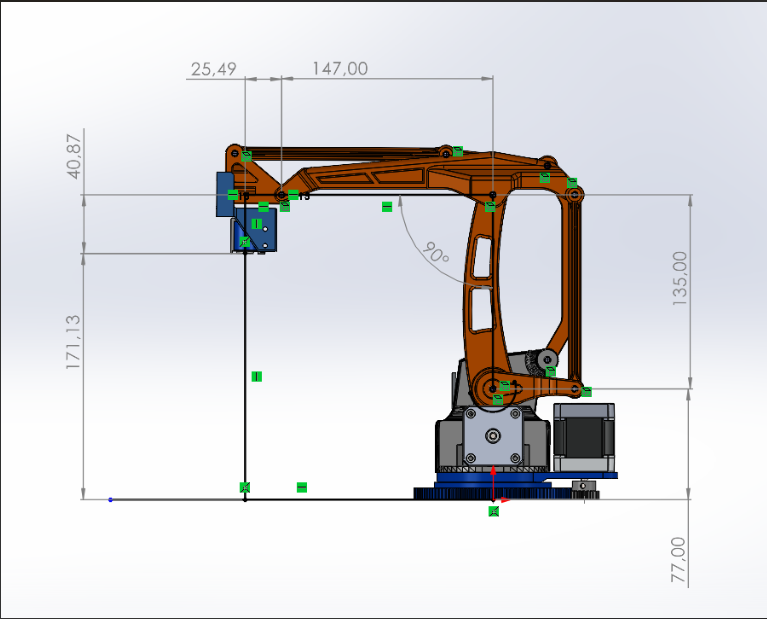
\includegraphics[width=0.8\textwidth]{Imagenes/Dimensiones.png}
    \caption{Validación de parámetros geométricos y offsets del manipulador en SolidWorks.}
    \label{fig:cinematica_solidworks}
\end{figure}

\subsection{Cinemática Directa (FK)}
Conocidos los ángulos articulares absolutos $Q_1$, $Q_2$ y $Q_3$, la posición cartesiana $(X, Y, Z)$ del efector final se obtiene proyectando los eslabones sobre el plano de trabajo. El radio total $R$ incorpora de manera directa el offset radial:

\begin{equation}
    R = L_2 \cos(Q_2) + L_3 \cos(Q_3) + O_r
\end{equation}

A partir de este radio, las coordenadas espaciales resultan en:

\begin{align}
    X &= R \cos(Q_1) \\
    Y &= R \sin(Q_1) \\
    Z &= L_1 + L_2 \sin(Q_2) + L_3 \sin(Q_3) - O_z
\end{align}

\subsection{Cinemática Inversa (IK)}
Dada una coordenada cartesiana objetivo $(X, Y, Z)$, el ángulo de la base se determina por proyección directa en el plano horizontal:

\begin{equation}
    Q_1 = \text{atan2}(Y, X)
\end{equation}

Para resolver el mecanismo en el plano vertical, se define el desplazamiento hacia el nodo de la muñeca restando los offsets constructivos:

\begin{align}
    r &= \sqrt{X^2 + Y^2} - O_r \\
    z' &= Z + O_z - L_1
\end{align}

La distancia lineal $D$ entre la articulación del hombro y la muñeca resulta en:

\begin{equation}
    D = \sqrt{r^2 + (z')^2}
\end{equation}

Aplicando el Teorema del Coseno al triángulo físico formado por los eslabones $L_2$, $L_3$ y la distancia $D$, se obtienen los ángulos internos $\beta$ y $\gamma$:

\begin{align}
    \beta &= \arccos\left(\frac{D^2 + L_2^2 - L_3^2}{2 \cdot D \cdot L_2}\right) \\
    \gamma &= \arccos\left(\frac{D^2 + L_3^2 - L_2^2}{2 \cdot D \cdot L_3}\right)
\end{align}

Conociendo el ángulo de elevación de $D$ respecto a la horizontal, definido como $\alpha = \text{atan2}(z', r)$, los ángulos absolutos de las articulaciones quedan definidos por las siguientes expresiones, garantizando implícitamente la configuración ``codo arriba'':

\begin{align}
    Q_2 &= \alpha + \beta \\
    Q_3 &= \alpha - \gamma
\end{align}

\begin{figure}[H]
    \centering
    \begin{tikzpicture}[scale=1.5, >=stealth, font=\sffamily, thick]
        \def\Qtwo{55}
        \def\Qthree{-30}
        \def\Ltwo{3.0}
        \def\Lthree{3.2}
        
        \coordinate (O) at (0,0);
        \coordinate (E) at (\Qtwo:\Ltwo);
        \coordinate (W) at ($(E) + (\Qthree:\Lthree)$);
        
        \draw[->, gray, thin] (-0.5, 0) -- (5.5, 0) node[right, black] {$r$};
        \draw[->, gray, thin] (0, -0.5) -- (0, 4.0) node[above, black] {$z'$};
        
        \draw[dashed, blue!80!black, line width=1pt] (O) -- (W) node[midway, below=2pt] {$D$};
        \draw[orange!90!black, line width=2.5pt] (O) -- (E) node[midway, above left] {$L_2$};
        \draw[orange!90!black, line width=2.5pt] (E) -- (W) node[midway, above right] {$L_3$};
        
        \draw[dashed, gray, thin] (E) -- ++(2,0);
        
        \pgfmathanglebetweenpoints{\pgfpointorigin}{\pgfpointanchor{W}{center}}
        \pgfmathsetmacro{\alphaAngle}{\pgfmathresult}
        
        \draw[->, red!70!black] (0.7,0) arc (0:\Qtwo:0.7) node[midway, right=1pt] {$Q_2$};
        \draw[->, green!50!black] (1.4,0) arc (0:\alphaAngle:1.4) node[midway, right=1pt] {$\alpha$};
        \draw[->, purple] (\alphaAngle:2.0) arc (\alphaAngle:\Qtwo:2.0) node[midway, right=1pt] {$\beta$};
        
        \draw[->, red!70!black] ($(E) + (0.9,0)$) arc (0:\Qthree:0.9) node[midway, right=2pt] {$Q_3$};
        
        \pgfmathsetmacro{\gammaStart}{\Qthree + 180}
        \pgfmathsetmacro{\gammaEnd}{\alphaAngle + 180}
        \draw[<-, purple] ($(W) + (\gammaStart:0.6)$) arc (\gammaStart:\gammaEnd:0.6) node[midway, left=2pt] {$\gamma$};
        
        \filldraw[fill=white, draw=black, line width=1pt] (O) circle (0.06) node[below left=2pt] {Hombro $(0,0)$};
        \filldraw[fill=white, draw=black, line width=1pt] (E) circle (0.06) node[above=4pt] {Codo};
        \filldraw[fill=white, draw=black, line width=1pt] (W) circle (0.06) node[right=4pt] {Muñeca $(r, z')$};
        
    \end{tikzpicture}
    \caption{Diagrama trigonométrico de la Cinemática Inversa en el plano proyectado $r-z'$, mostrando las relaciones angulares de los eslabones.}
    \label{fig:diagrama_ik}
\end{figure}

\begin{figure}[H]
    \centering
    \begin{tikzpicture}[scale=1.5, >=stealth, font=\sffamily, thick]
        \def\alphaAng{35}
        \def\betaAng{45}
        \def\gammaAng{60}
        \def\Ltwo{3.5}
        
        \pgfmathsetmacro{\Lthree}{\Ltwo * sin(\betaAng) / sin(\gammaAng)}
        
        \pgfmathsetmacro{\Qtwo}{\alphaAng + \betaAng}
        \pgfmathsetmacro{\Qthree}{\alphaAng - \gammaAng}
        
        \coordinate (O) at (0,0);
        \coordinate (E) at (\Qtwo:\Ltwo);
        \coordinate (W) at ($(E) + (\Qthree:\Lthree)$);
        
        \draw[dashed, gray, thin] (-0.5,0) -- (4.5,0);
        \draw[dashed, gray, thin] ($(E) + (-1,0)$) -- ($(E) + (3,0)$);
        
        \draw[dashed, blue, line width=1pt] (O) -- (W) node[midway, below right] {$D$};
        \draw[dashed, blue, line width=1pt] (E) -- ($(E) + (\alphaAng:2.5)$) coordinate (E_parallel);
        
        \draw[orange!90!black, line width=2.5pt] (O) -- (E) node[midway, above left] {$L_2$};
        \draw[orange!90!black, line width=2.5pt] (E) -- (W) node[midway, below left] {$L_3$};
        
        \draw[->, green!50!black] (1.2,0) arc (0:\alphaAng:1.2) node[midway, right=1pt] {$\alpha$};
        \draw[->, purple] (\alphaAng:1.6) arc (\alphaAng:\Qtwo:1.6) node[midway, above right=-2pt] {$\beta$};
        
        \draw[->, green!50!black] ($(E) + (1.2,0)$) arc (0:\alphaAng:1.2) node[midway, right=1pt] {$\alpha$};
        \draw[<-, purple] ($(E) + (\Qthree:1.8)$) arc (\Qthree:\alphaAng:1.8) node[midway, right=1pt] {$\gamma$};
        \draw[->, red!70!black] ($(E) + (0.8,0)$) arc (0:\Qthree:0.8) node[midway, right=1pt] {$Q_3$};
        
        \filldraw[fill=white, draw=black, line width=1pt] (O) circle (0.06) node[below left] {Hombro $(O)$};
        \filldraw[fill=white, draw=black, line width=1pt] (E) circle (0.06) node[above=4pt] {Codo $(E)$};
        \filldraw[fill=white, draw=black, line width=1pt] (W) circle (0.06) node[below=4pt] {Muñeca $(W)$};
        
    \end{tikzpicture}
    \caption{Demostración visual del ángulo $Q_3$. Al trazar una línea paralela a $D$ desde el Codo, se observa por ángulos alternos internos que la inclinación absoluta del antebrazo es $Q_3 = \alpha - \gamma$.}
    \label{fig:demostracion_q3}
\end{figure}

\section{Reingeniería de acoples mecánicos (Unión por chavetero)}
Con el fin de resolver los problemas de deslizamiento y holgura torsional detectados en los acoples originales del sistema heredado, se llevó a cabo una reingeniería integral de la transmisión mecánica. Esta intervención consistió en el mecanizado de los ejes cilíndricos de los motores paso a paso para incorporar un alojamiento preciso, combinado con el rediseño y fabricación de los engranajes plásticos impresos en 3D para integrar una unión por chaveta. Esta solución proporciona una transmisión de torque rígida y mitiga de forma sustancial las desalineaciones angulares durante la operación continua de los ejes.

\begin{figure}[H]
    \centering
    \begin{subfigure}[b]{0.48\textwidth}
        \centering
        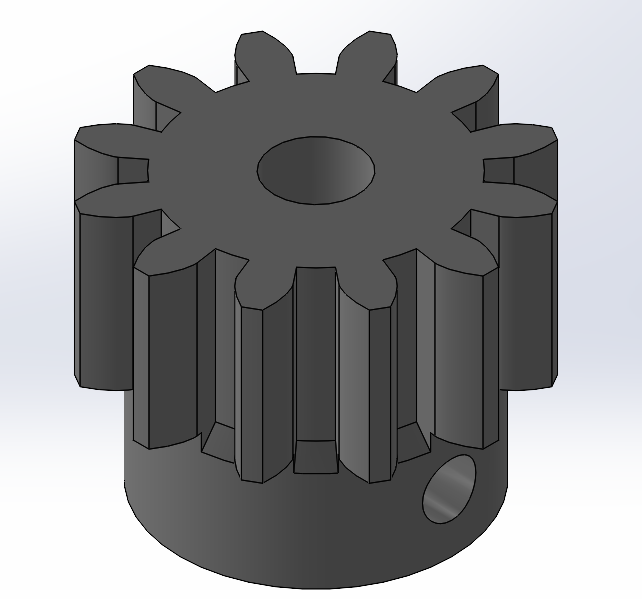
\includegraphics[width=\textwidth]{Imagenes/engranajeAnterior.png} 
        \caption{Engranaje original con acople por fricción.}
        \label{fig:engranaje_anterior}
    \end{subfigure}
    \hfill
    \begin{subfigure}[b]{0.48\textwidth}
        \centering
        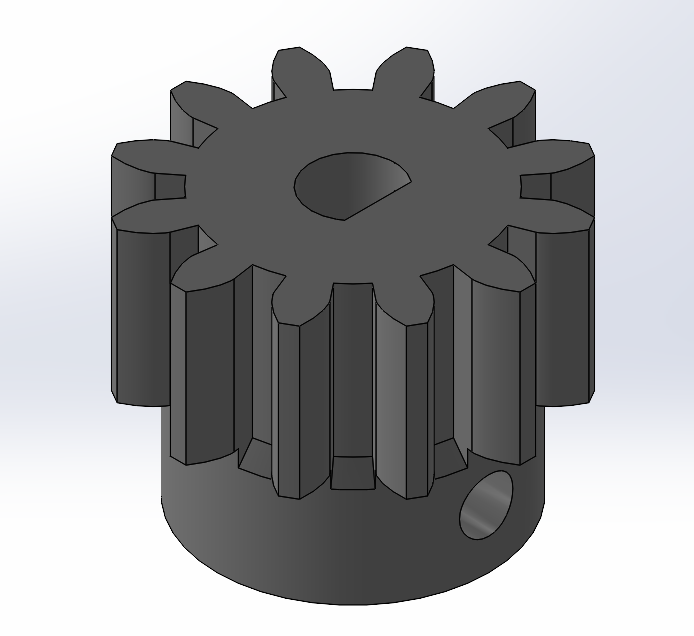
\includegraphics[width=\textwidth]{Imagenes/engranajeModificado.png} 
        \caption{Engranaje impreso en 3D con unión por chaveta.}
        \label{fig:engranaje_chaveta}
    \end{subfigure}
    \caption{Comparativa de la reingeniería mecánica de engranajes.}
    \label{fig:reingenieria_mecanica}
\end{figure}

\section{Optimización de la integridad de señal en buses I2C}
Durante las pruebas iniciales del sistema, se detectaron anomalías e intermitencias en la comunicación con los sensores magnéticos basados en el protocolo I2C. Tras una revisión detallada del hardware, se identificó que el arnés de cables original presentaba una disposición física desfavorable: las líneas de reloj (\textit{SCL}) y de datos (\textit{SDA}) se encontraban trenzadas entre sí. Esta disposición propicia el acoplamiento capacitivo y la diafonía (\textit{cross-talk}) mutua entre señales digitales de alta frecuencia.

Para reducir el ruido electromagnético inducido y asegurar la estabilidad del bus, se rediseñó el tendido separando las líneas de señal y aplicando un esquema de par trenzado de referencia cerrada: se trenzó de manera independiente la línea de reloj con la referencia a tierra (\textit{SCL} con \textit{GND}), y la línea de datos con la alimentación (\textit{SDA} con \textit{VCC}). Esta modificación atenuó notablemente la susceptibilidad al ruido eléctrico generado por la conmutación de los motores paso a paso, logrando una transmisión de datos estable en el rango operativo del manipulador.

\section{Implementación del Nodo de Visión Artificial y Calibración}
Para dotar al sistema de la capacidad de percibir su entorno, se desarrolló un nodo de visión dedicado en ROS 2 (\texttt{VisionDetectorNode}) integrado con OpenCV, tomando como base arquitecturas de percepción aplicadas a brazos robóticos industriales \cite{bib:vo}. Este subsistema procesa el flujo de video en tiempo real de una cámara cenital conectada mediante un enlace persistente (\textit{symlink}). Dado que las condiciones de iluminación ambiental afectan de forma directa la segmentación cromática, el desarrollo contempló herramientas de calibración que favorecen la repetibilidad del sistema:

    \subsection{Calibración Dinámica y Umbrales en Espacio HSV:} 
    Mediante una interfaz auxiliar interactiva (\texttt{calibrar\_hsv.py}) provista de controles deslizantes (\textit{trackbars}), es posible sintonizar de forma dinámica los rangos cromáticos del espacio de color HSV (Tono, Saturación y Valor). Esta transformación desacopla la información de color de la intensidad lumínica ambiental, aislando con alta fidelidad la silueta del objeto de prueba respecto al fondo de la cinta. 
    
    Para purificar la máscara binaria resultante y eliminar los falsos positivos derivados del ruido del sensor o de reflejos en la superficie de la banda, se implementa una secuencia estricta de filtros morfológicos en dos etapas utilizando elementos estructurantes (\textit{kernels}):
    \begin{enumerate}
        \item \textbf{Operación de Cierre (\textit{Morphological Close}):} Se aplica un kernel rectangular de $11\times11$ píxeles de manera iterativa (2 pasadas). Esta operación ejecuta una dilatación seguida de una erosión, lo que permite rellenar pequeños huecos, discontinuidades u oclusiones internas dentro de la silueta segmentada del objeto, asegurando un contorno cerrado y sólido.
        \item \textbf{Operación de Apertura (\textit{Morphological Open}):} A continuación, se aplica un kernel de menor tamaño de $5\times5$ píxeles. Consiste en una erosión seguida de una dilatación, destinada a suprimir el ruido disperso de fondo (pequeños puntos o motas aisladas que superan el umbral de color pero no pertenecen a una pieza válida).
    \end{enumerate}
\subsection{Extracción del Centroide y Publicación en ROS 2}
Una vez aplicada la máscara de color y filtrado el ruido mediante operaciones morfológicas de apertura y cierre, el nodo analiza los contornos presentes en la escena. Al detectar el objeto de mayor área por encima del umbral establecido, se calculan los momentos espaciales de la imagen mediante la función \texttt{cv2.moments()}. A partir de los momentos de orden cero y uno, se obtiene la posición del centroide en píxeles $(cx, cy)$ aplicando las expresiones:

\begin{equation}
cx = \frac{M_{10}}{M_{00}}, \quad cy = \frac{M_{01}}{M_{00}}
\label{eq:centroide}
\end{equation}

donde $M_{00}$ representa el área total del objeto (momento de orden cero), y $M_{10}$ y $M_{01}$ son los momentos espaciales de primer orden respecto a los ejes $X$ e $Y$, respectivamente.

Esta posición en píxeles es convertida a coordenadas métricas utilizando el modelo polinómico cuadrático calibrado. Finalmente, el nodo empaqueta estas coordenadas espaciales en mensajes estándar de ROS 2 del tipo \texttt{geometry\_msgs/Point} y los transmite mediante dos publicadores: uno de flujo continuo para el modo estático y otro síncrono para las rutinas dinámicas del manipulador.

    \subsection{Mapeo Métrico por Ajuste Polinómico (Píxel a Milímetro):} Para traducir las coordenadas de imagen desde el sistema de píxeles hacia unidades métricas reales en la base del robot, se implementó una rutina de calibración espacial. Este procedimiento se realiza posicionando el efector final a lo largo de la cinta transportadora mediante la cinemática directa (\textit{FK}) de la interfaz gráfica en un rango de $[-140, 140]\text{ mm}$ sobre el eje $Y$ del robot. 
    
    Mediante el script \texttt{capturar\_punto.py}, se obtienen las coordenadas centroidales en píxeles de la cámara (correspondientes a la posición horizontal $x$ en la imagen) asociadas a cada posición real conocida. A partir de estos datos, recopilados en la Tabla~\ref{tab:obtension_puntos_calibracion}, se emplea el script de automatización \texttt{calcular\_polinomico.py}. Este programa interactivo procesa los pares empíricos aplicando un modelo de regresión por mínimos cuadrados mediante la función \texttt{np.polyfit()} de NumPy, resolviendo un polinomio de segundo orden de la forma $Y_{\text{robot}} = a \cdot X_{\text{px}}^2 + b \cdot X_{\text{px}} + c$. Su ejecución permite calcular con alta precisión los coeficientes empíricos que compensan los errores de curvatura y distorsión óptica de la lente cenital, garantizando linealidad métrica en todo el trayecto útil sobre la banda.
\begin{table}[H]
\centering
\small
\begin{tabular}{|c|c|c|}
\hline
\textbf{Punto N$^\circ$} & \textbf{$Y_{\text{real}}$ [mm]} & \textbf{Coordenada $X$ [píxeles]} \\ \hline
1  & -139.4 & 539.51 \\ \hline
2  & -119.7 & 512.61 \\ \hline
3  & -99.3  & 478.64 \\ \hline
4  & -79.4  & 445.67 \\ \hline
5  & -60.3  & 413.91 \\ \hline
6  & -40.0  & 383.16 \\ \hline
7  & -20.1  & 354.19 \\ \hline
8  &   0.3  & 318.16 \\ \hline
9  &  19.8  & 287.23 \\ \hline
10 &  40.1  & 250.50 \\ \hline
11 &  60.0  & 217.86 \\ \hline
12 &  79.8  & 184.59 \\ \hline
13 &  99.1  & 153.92 \\ \hline
14 & 119.8  & 122.78 \\ \hline
15 & 139.5  &  89.47 \\ \hline
\end{tabular}
\caption{Registro completo de adquisición de puntos experimentales para la calibración espacial ($N = 15$).}
\label{tab:obtension_puntos_calibracion}
\end{table}

\begin{figure}[H]
\centering
\begin{tikzpicture}
\begin{axis}[
    width=0.85\textwidth,
    height=6.5cm,
    xlabel={Coordenada Horizontal $X$ [píxeles]},
    ylabel={Posición Real $Y_{\text{FK}}$ [mm]},
    grid=major,
    grid style={dashed, gray!30},
    xmin=50, xmax=580,
    ymin=-160, ymax=160,
    legend pos=north west,
    font=\small
]

    % Curva de tendencia cuadrática superpuesta (Modelo del nodo de visión)
    \addplot[
        domain=74.91:553.78,
        samples=100,
        color=primary,
        thick,
        smooth
    ] {0.0000278487 * x^2 + 0.5997512673 * x -193.5175741780};
    \addlegendentry{Modelo Polinómico Cuadrático}

    % Puntos experimentales registrados en la Tabla (N = 15)
    \addplot[
        only marks,
        mark=*,
        mark size=2pt,
        color=accentred
    ] coordinates {
        (89.47, -140.63)
        (122.78, -120.41)
        (153.92, -100.22)
        (184.59, -79.89)
        (217.86, -60.16)
        (250.50, -40.28)
        (287.23, -20.86)
        (318.16, 0.34)
        (354.19, 20.14)
        (383.16, 40.37)
        (413.91, 60.20)
        (445.67, 79.57)
        (478.64, 99.60)
        (512.61, 120.25)
        (539.51, 139.48)
        
    };
    \addlegendentry{Puntos Experimentales N 15}

\end{axis}
\end{tikzpicture}
\caption{Curva de calibración polinómica $Y_{\text{FK}}$ frente a $X$ en píxeles, evidenciando la mitigación de la distorsión óptica.}
\label{fig:curva_calibracion_experimental}
\end{figure}

    


\subsection{Test Experimental y Análisis de Dispersión del Sistema de Visión}
Para cuantificar rigurosamente la precisión métrica del nodo de visión una vez implementado el ajuste polinómico cuadrático, se desarrolló una serie de pruebas sistemáticas directamente sobre la maqueta física de la celda, basándose en la captura de $N = 15$ puntos de control distribuidos longitudinalmente sobre la cinta transportadora.

\textbf{Metodología del Ensayo:} Utilizando la cinemática directa (FK) desde la interfaz gráfica de usuario (GUI), se posicionó de manera estática el efector final con un cubo de referencia patrón en marcas espaciadas cada $20.0\text{ mm}$ de forma sucesiva, abarcando todo el rango operativo de la cinta desde $Y = -140.0\text{ mm}$ hasta $Y = +140.0\text{ mm}$. En cada una de las 15 posiciones discretas, el nodo \texttt{VisionDetectorNode} procesó la imagen para estimar la coordenada cartesiana $\hat{Y}$ mediante el modelo polinómico, registrando el desvío residual absoluto $e_i = |\hat{Y}_i - Y_{\text{real}, i}|$.

\begin{table}[H]
\centering
\small
\begin{tabular}{|c|c|c|c|}
\hline
\textbf{Punto N$^\circ$} & \textbf{$Y_{\text{real}}$ [mm]} & \textbf{$Y_{\text{vision}}$ [mm]} & \textbf{Error Residual $e_i$ [mm]} \\ \hline
1  & -139.4 & -137.8 & 1.6 \\ \hline
2  & -119.7 & -118.0  & 1.7 \\ \hline
3 & -99.3  & -98.3  & 1.0 \\ \hline
4 & -79.4    & -79.2   & 0.2 \\ \hline
5 & -60.3 & -60.2  & 0.1 \\ \hline
6 & -40.0 & -39.6 & 0.4 \\ \hline
7 & -20.1 & -19.6 & 0.5 \\ \hline
8  & 0.3 & 0.5 & 0.2 \\ \hline
9  & 19.8 & 20.7  & 0.9 \\ \hline
10 & 40.1  & 40.6  & 0.5 \\ \hline
11 & 60.0    & 59.3   & 0.7 \\ \hline
12 & 79.8  & 79.5  & 0.3 \\ \hline
13 & 99.1 & 99.7 & 0.6 \\ \hline
14 & 119.8 & 118.7 & 1.1 \\ \hline
15 & 139.5 & 140.0 & 0.5 \\ \hline
\end{tabular}
\caption{Muestra representativa del test de dispersión del sistema de visión ($N = 15$ puntos muestreados cada $20\text{ mm}$).}
\label{tab:test_vision_dispersion}
\end{table}

\textbf{Análisis Estadístico de Dispersión y Errores:}
A partir de la serie completa de los 15 puntos registrados experimentalmente, se computaron los indicadores globales de desempeño del algoritmo de percepción:
\begin{itemize}
    \item \textbf{Error Medio (Bias):} $+0.41\text{ mm}$
    \item \textbf{Error Absoluto Medio (MAE):} $0.69\text{ mm}$
    \item \textbf{Raíz del Error Cuadrático Medio (RMSE):} $0.83\text{ mm}$
    \item \textbf{Desviación Estándar de Dispersión ($\sigma$):} $0.73\text{ mm}$
    \item \textbf{Error Máximo Residual:} $1.70\text{ mm}$
\end{itemize}

Los resultados cuantitativos demuestran que la dispersión del sistema de visión se mantiene dentro de una cota submilimétrica en la región central del campo visual y no supera $1.70\text{ mm}$ en los extremos del área de trabajo. Esta baja dispersión ($\sigma = 0.73\text{ mm}$) certifica la alta repetibilidad del nodo de visión y valida la suficiencia del modelo cuadrático para mitigar la distorsión óptica de la lente cenital, asegurando un posicionamiento altamente compatible con la tolerancia de agarre del efector magnético.
\subsection{Clasificación Geométrica de Objetos Invariante a la Rotación}
Para habilitar la capacidad de clasificación del sistema, se integró un algoritmo capaz de discriminar entre distintas geometrías de piezas que comparten el mismo color (en este caso, un cubo y un cono truncado de color rosa).

La discriminación basada únicamente en contornos básicos resultaba sensible ante sombras o variaciones de silueta. Inicialmente se evaluó el método del \textbf{Extent Rotado} (relación entre el área del objeto y su \texttt{minAreaRect}). No obstante, las pruebas experimentales demostraron que cuando el cubo ingresaba orientado en diagonal, el filtrado morfológico redondeaba sus esquinas, reduciendo su coeficiente Extent a valores cercanos a los del cono ($\approx 0.81$).

Para resolver este solapamiento y alcanzar una alta tasa de discriminación geométrica independiente de la orientación, se incorporó una segunda métrica basada en la \textbf{Relación de Cajas (Rect Ratio)}:

\begin{equation}
    \text{Rect Ratio} = \frac{A_{\text{rotada}}}{A_{\text{recta}}} = \frac{\text{Área } \texttt{minAreaRect}}{\text{Área } \texttt{boundingRect}}
\end{equation}

La lógica de decisión combinada opera evaluando la dispersión de área: si el cubo se encuentra rotado, su caja recta encierra una mayor proporción de fondo vacío, produciendo un \textit{Rect Ratio} inferior a $0.85$. Si la pieza transita alineada con la cinta, ambas cajas presentan áreas semejantes (\textit{Rect Ratio} $\approx 1.0$), instancia en la cual se evalúa su densidad mediante el \textit{Extent} (donde un cubo presenta valores sistemáticamente mayores a $0.85$). Este enfoque complementario otorga una clasificación geométrica confiable frente a distintas orientaciones de ingreso de la pieza.

\begin{figure}[H]
    \centering
    \begin{subfigure}[b]{0.48\textwidth}
        \centering
        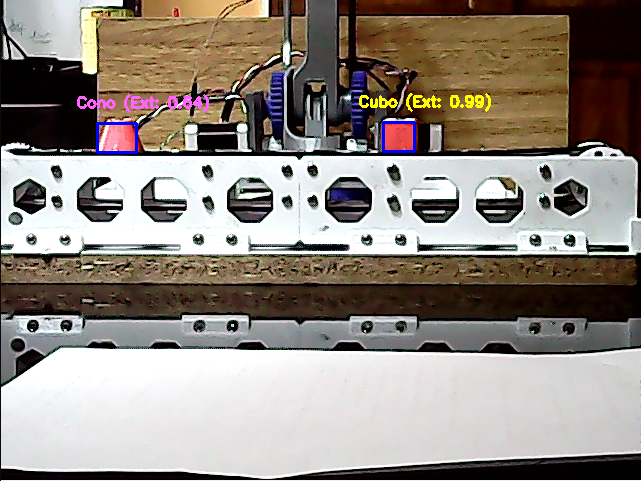
\includegraphics[width=\textwidth]{Imagenes/captura_camara_clasificacion.png} 
        \caption{Vista de cámara con caja rotada (\texttt{minAreaRect}) y clasificación por Extent.}
        \label{fig:captura_clasificacion}
    \end{subfigure}
    \hfill
    \begin{subfigure}[b]{0.48\textwidth}
        \centering
        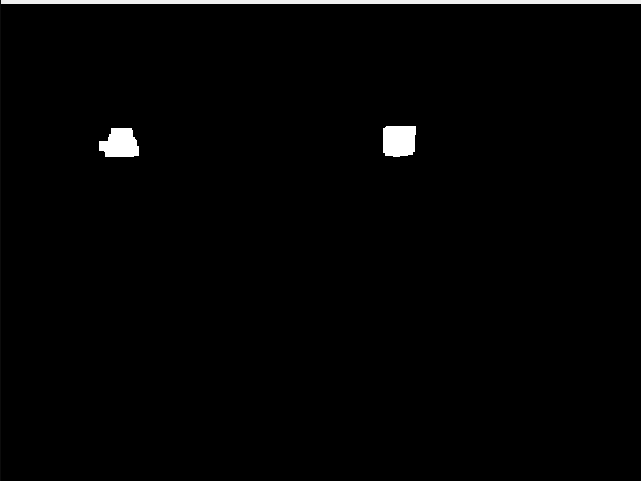
\includegraphics[width=\textwidth]{Imagenes/captura_mascara_clasificacion.png} 
        \caption{Máscara HSV segmentada, evidenciando las diferentes geometrías.}
        \label{fig:mascara_clasificacion}
    \end{subfigure}
    \caption{Clasificación simultánea de geometrías mediante el cálculo del Extent Rotado.}
    \label{fig:clasificacion_objetos}
\end{figure}

\section{Diseño e Implementación de la Interfaz Gráfica de Usuario (GUI)}
Con el fin de centralizar la supervisión y operación de la celda robótica, se desarrolló una interfaz gráfica de usuario desde cero utilizando el framework \textbf{PyQt5}, estructurada en un entorno modular de cinco pestañas principales adaptadas a las distintas fases de experimentación y control. Las Pestañas 2 y 3 están destinadas a la configuración interna de parámetros y telemetría articular, enfocando la operación de la celda en las Pestañas 1, 4 y 5.

\begin{itemize}
    \item \textbf{Pestaña 1 (Control Manual y P2P):} Diseñada para la operación directa y el posicionamiento manual del manipulador (ver Figura~\ref{fig:gui_pestana1}). Incorpora deslizadores y selectores numéricos con validación de límites articulares para el envío de consignas punto a punto ejecutadas mediante temporizadores en el firmware. Incluye además un cuadro de entrada para coordenadas cartesianas $(X, Y, Z)$ validadas mediante cinemática inversa, interruptores para el accionamiento del solenoide, secuencia de \textit{homing} y botón de parada por software.

    \begin{figure}[H]
        \centering
        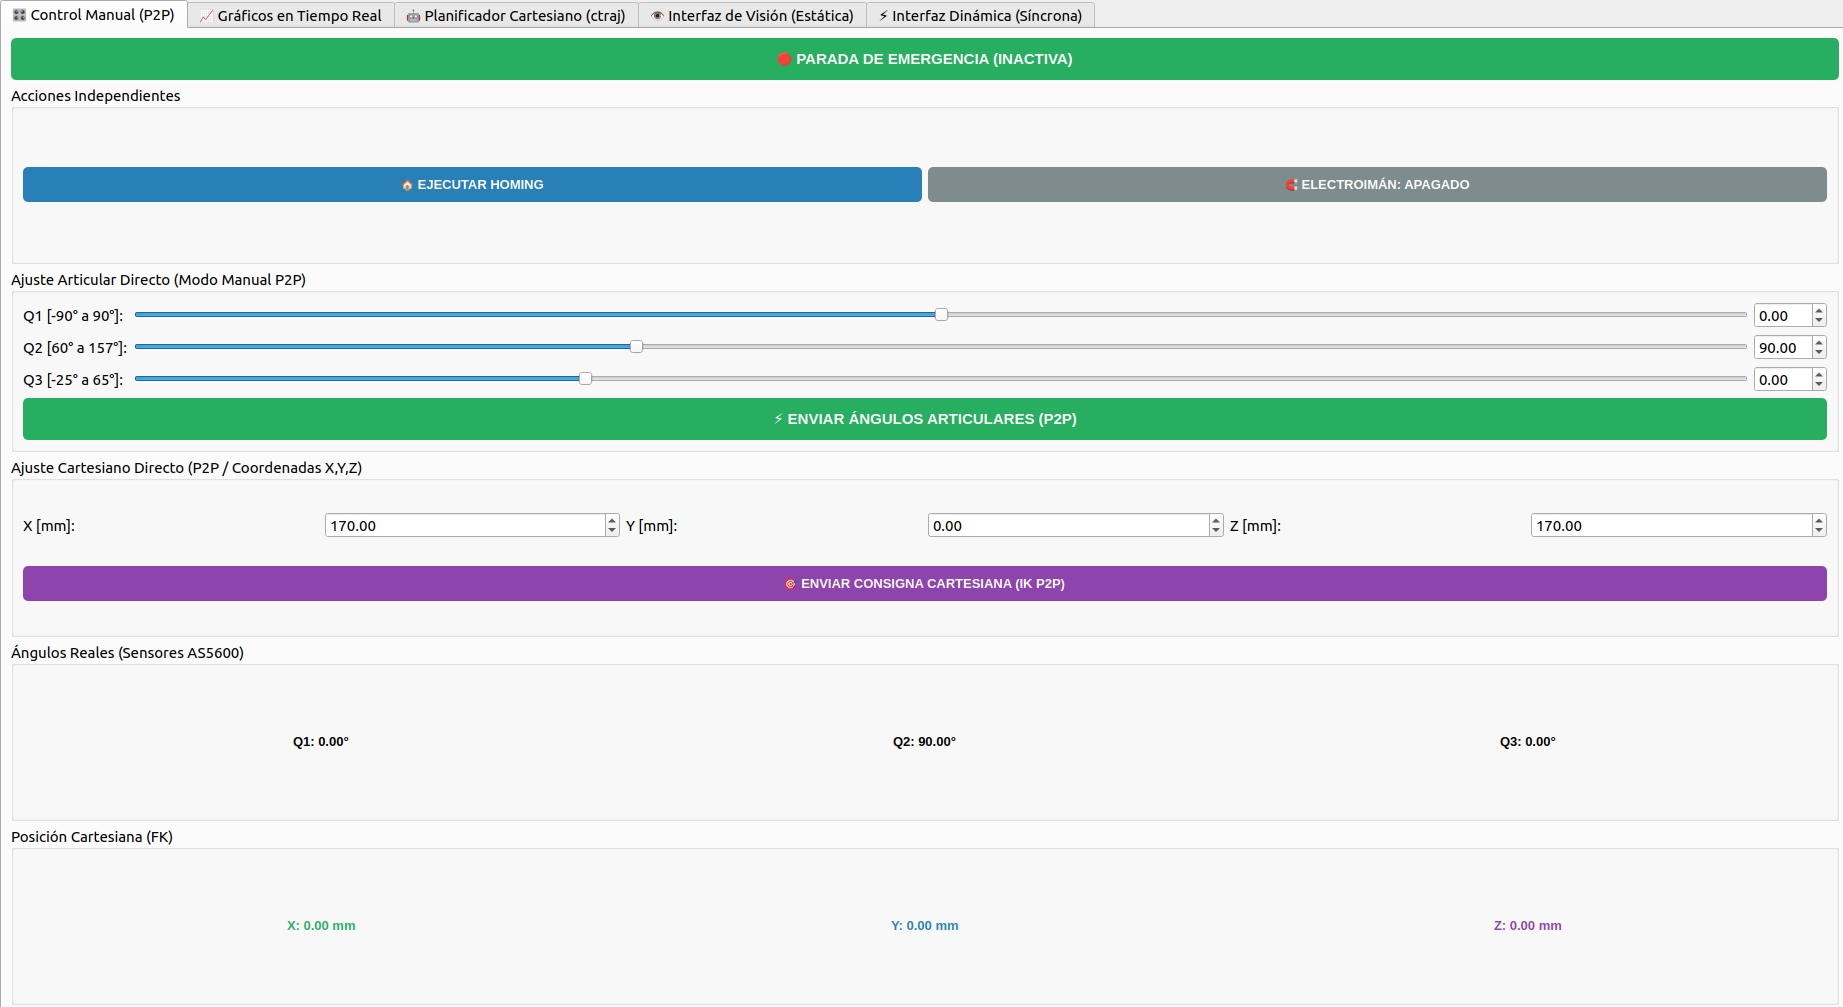
\includegraphics[width=0.95\textwidth]{Imagenes/gui_pestana1.png}
        \caption{Vista general de la Pestaña 1: Control manual, sliders articulares y panel de consignas cartesianas.}
        \label{fig:gui_pestana1}
    \end{figure}
    
    \item \textbf{Pestaña 4 (Pick Estático):} Destinada a la validación de la celda de clasificación con piezas en reposo (ver Figura~\ref{fig:gui_pestana4}). El módulo de visión artificial detecta un cubo de referencia de $20\text{ mm}$ de lado ($20\times 20\times 20\text{ mm}$) de color rosa y transmite un vector de posición cartesiano $(x, y, z)$ hacia el planificador embebido. Las coordenadas nominales efectivas se establecieron en la cota $Z = 78.0\text{ mm}$ y posición longitudinal de cinta $X = 215.0\text{ mm}$.

    \begin{figure}[H]
        \centering
        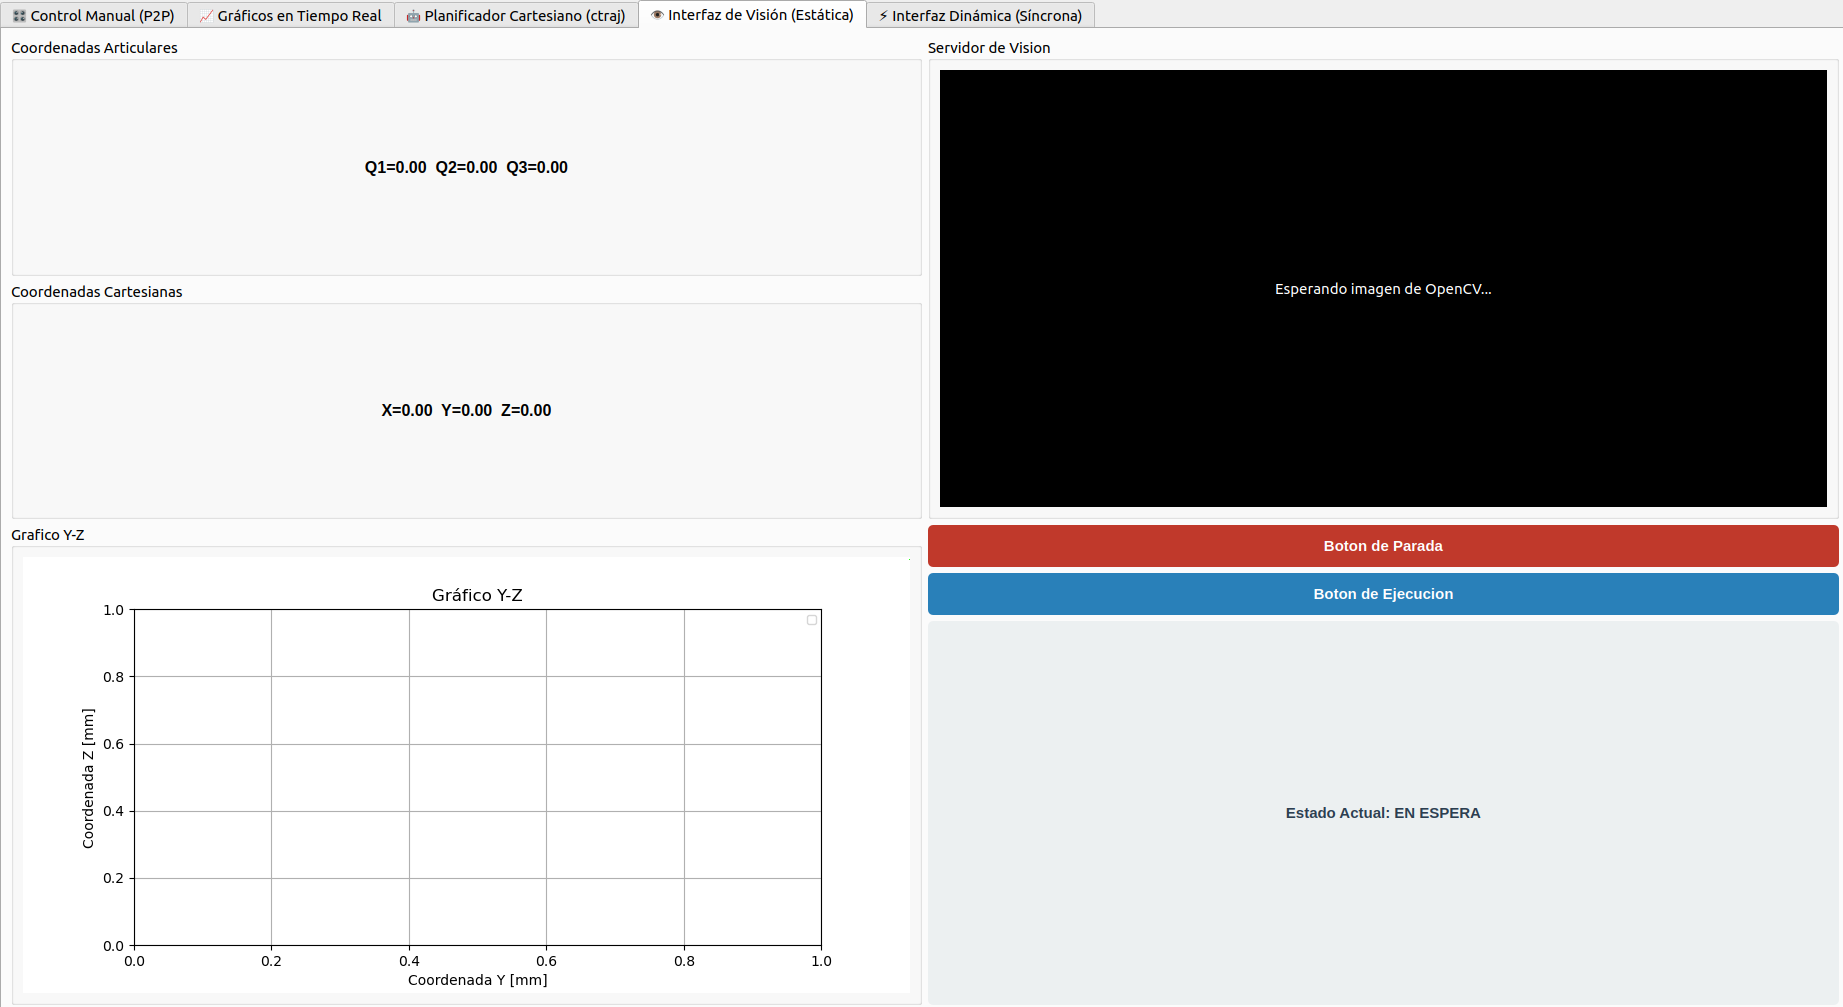
\includegraphics[width=0.95\textwidth]{Imagenes/gui_pestana4.png}
        \caption{Vista de la Pestaña 4: Ensayo de clasificación Pick-and-Place estático con retroalimentación visual.}
        \label{fig:gui_pestana4}
    \end{figure}
    
    \item \textbf{Pestaña 5 (Pick Dinámico y Síncrono V1):} Implementó la primera aproximación operativa para la manipulación de piezas en movimiento sobre la cinta transportadora (ver Figura~\ref{fig:gui_pestana5}). La arquitectura de software se estructuró sobre una máquina de estados determinista que dividió el ciclo en las siguientes etapas operativas:
    \begin{enumerate}
        \item \textbf{Calibración Cinemática de la Cinta:} Para estimar la velocidad lineal constante del objeto, se implementó un algoritmo de medición basado en compuertas de tiempo virtuales sobre el flujo de video. Al activar el comando de calibración desde la interfaz, el nodo de visión define dos fronteras espaciales a lo largo del eje longitudinal, separadas por una distancia física conocida de $\Delta Y = 290\text{ mm}$. El sistema monitorea el centroide de la pieza; al cruzar la primera compuerta se registra una estampa de tiempo inicial ($t_1$). Al intersectar la segunda compuerta, se captura el tiempo final ($t_2$), obteniendo el diferencial temporal $\Delta t = t_2 - t_1$. Finalmente, la velocidad escalar se calcula como $V = \Delta Y / \Delta t$, valor que es transmitido y almacenado globalmente en la máquina de estados para alimentar el modelo predictivo.
        
        \item \textbf{Posicionamiento en Guardia y Lazo de Tolerancia:} Previo a la intercepción, el brazo manipulador era comandado hacia una posición de guardia estratégica (e.g., $X=215, Y=-75, Z=100\text{ mm}$). El algoritmo validaba el arribo del efector final evaluando el error euclídeo en los tres ejes, requiriendo que la posición real se encontrara dentro de una estricta esfera de tolerancia de $\pm2.0\text{ mm}$. Una vez superada esta condición, se energizaba el electroimán de forma anticipada.
        
        \item \textbf{Cálculo Predictivo MRU e Intercepción Síncrona:} Con el manipulador en guardia, el sistema evaluaba continuamente la coordenada longitudinal entrante del objeto ($Y_{actual}$). En lugar de un seguimiento reactivo ciego, el algoritmo predecía el punto temporal exacto de captura asumiendo un Movimiento Rectilíneo Uniforme (MRU): 
        \begin{equation}
            t_{objetivo} = \left( \frac{Y_{pick} - Y_{actual}}{V} \right) - T_{anticipo}
        \end{equation}
        donde $Y_{pick}$ ($120\text{ mm}$) representa la coordenada longitudinal fija de intercepción, y $T_{anticipo}$ ($0.15\text{ s}$) compensa el retardo de saturación magnética del solenoide. Siempre que el $t_{objetivo}$ respetara el límite de aceleración física del robot ($t \ge 0.85\text{ s}$), se generaba una trayectoria polinómica quíntica que sincronizaba temporal y espacialmente el contacto entre el cabezal y la pieza.
    \end{enumerate}

 
    \begin{figure}[H]
        \centering
        \begin{tikzpicture}[
            % Definición de distancias entre nodos
            node distance=0.7cm and 1cm,
            % Estilos de las cajas y flechas
            process/.style={rectangle, draw=gray!80!black, thick, minimum width=4.5cm, minimum height=1cm, text centered, font=\sffamily\small, align=center},
            decision/.style={diamond, draw=gray!80!black, thick, minimum width=4.5cm, minimum height=1.5cm, text centered, font=\sffamily\small, align=center, aspect=1.5},
            arrow/.style={thick, ->, >=Stealth, draw=black},
            labelbox/.style={fill=gray!30, inner sep=2pt, font=\sffamily\scriptsize}
            ]

            % Nodos
            \node (start) [process] {Inicio: Visión / GUI};
            \node (btnvel) [process, below=of start] {Botón: Medir Velocidad};
            \node (camara) [process, below=of btnvel] {Cámara detecta recorrido \\ de 290 mm};
            \node (vmed) [process, below=of camara] {V medida = constante};
            \node (calc) [process, below=of vmed] {Cálculo: t = (Xf - X0) / V};
            \node (btnpick) [process, below=of calc] {Botón: Pick};
            \node (posini) [process, below=of btnpick] {Posición Inicial: (220, -75, \\ 100)};
            \node (solenoide) [process, below=of posini] {Encender Solenoide};
            \node (detecta) [decision, below=of solenoide] {¿Se detecta cubo rosa?};
            \node (tomar) [process, below=of detecta] {Tomar coordenada Y0 y \\ calcular tiempo};
            \node (enviar) [process, below=of tomar] {Enviar tiempo al \\ microcontrolador para \\ mover el brazo};

            % Conexiones (Flechas principales)
            \draw [arrow] (start) -- (btnvel);
            \draw [arrow] (btnvel) -- (camara);
            \draw [arrow] (camara) -- (vmed);
            \draw [arrow] (vmed) -- (calc);
            \draw [arrow] (calc) -- (btnpick);
            \draw [arrow] (btnpick) -- (posini);
            \draw [arrow] (posini) -- (solenoide);
            \draw [arrow] (solenoide) -- (detecta);

            % Conexiones de decisión
            \draw [arrow] (detecta) -- node[labelbox] {Sí} (tomar);
            % Flecha de retorno curva para el "No"
            \draw [arrow] (detecta.140) to[bend left=20] node[labelbox, right, pos=0.4] {No} (solenoide.220);

            \draw [arrow] (tomar) -- (enviar);

        \end{tikzpicture}
        \caption{Diagrama de flujo del proceso de visión y control.}
        \label{fig:diagrama_flujo}
    \end{figure}


    \begin{figure}[H]
        \centering
        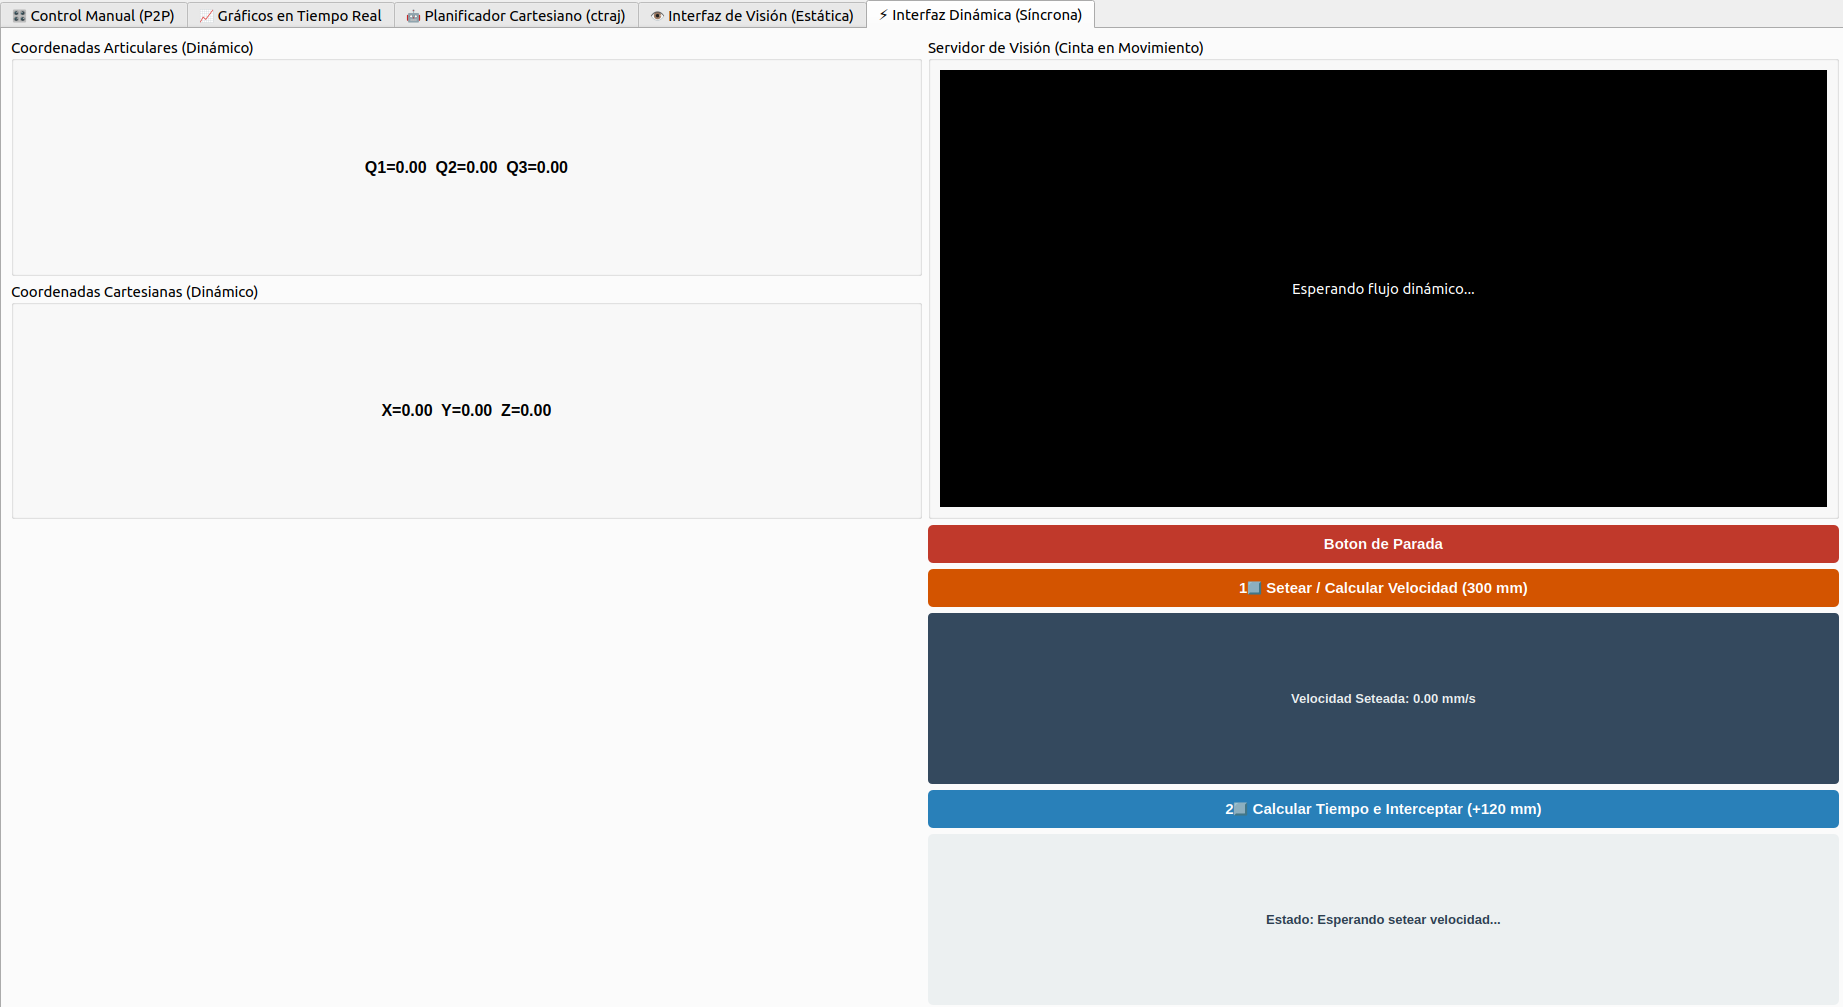
\includegraphics[width=0.95\textwidth]{Imagenes/gui_pestana5.png}
        \caption{Vista de la Pestaña 5: Ensayo de clasificación Pick-and-Place Dinámico.}
        \label{fig:gui_pestana5}
    \end{figure}
\end{itemize}

\section{Evolución hacia el Modo Dinámico Continuo en 1 Paso (V2)}
Para superar la dependencia del operador y optimizar los tiempos de ciclo, se llevó a cabo una reingeniería completa del lazo dinámico, implementada en una arquitectura modular desacoplada (\texttt{robot\_ui\_node\_2} y máquina de estados \texttt{PickAndPlaceSMV2}). Esta versión V2 sustituyó el esquema de dos etapas por un algoritmo continuo que estima la velocidad de cada pieza y ejecuta la trayectoria de intercepción de forma automática.

\subsection{Estimación de Velocidad por Compuertas Espaciales en Visión}
En los ensayos preliminares de la versión V1, calcular la velocidad en el hilo de la interfaz mediante la diferencia temporal de mensajes ROS 2 introducía desvíos notables (del orden del $20\text{--}25\%$) debido a la latencia acumulada en los buffers de captura de video y al retardo de refresco gráfico.

Para mitigar las fluctuaciones temporales (\textit{jitter}) y desacoplar la estimación de la carga de la interfaz, el cálculo de velocidad se trasladó al lazo de procesamiento en OpenCV dentro de \texttt{VisionDetectorNode}. Se establecieron dos compuertas espaciales virtuales fijas sobre la cinta:
\begin{itemize}
    \item \textbf{Compuerta de Entrada ($Y_1 = -160.0\text{ mm}$):} Registra la marca temporal de cruce $t_1$ mediante \texttt{time.perf\_counter()}.
    \item \textbf{Compuerta de Medición y Disparo ($Y_2 = -90.0\text{ mm}$):} Registra la marca temporal $t_2$ al completar el recorrido fijo $\Delta Y = 70.0\text{ mm}$.
\end{itemize}

La velocidad lineal estimada del objeto se obtiene directamente a partir del diferencial observado:
\begin{equation}
    v_{\text{obj}} = \frac{Y_2 - Y_1}{t_2 - t_1}
\end{equation}

Una vez validada la magnitud dentro de los límites operativos admisibles ($v_{\text{obj}} \in [40.0, 250.0]\text{ mm/s}$), el nodo publica la pose y velocidad a través de \texttt{/detected\_object\_dynamic\_pose}, activando de inmediato la máquina de estados.

\subsection{Modelo de Sincronización Temporal e Intercepción en $Y_{\text{pick}}$}
Al detectarse el cruce por la cota de disparo ($y_{\text{disparo}} = Y_2$), la distancia restante hasta el punto nominal de intercepción ($Y_{\text{pick}} = 120.0\text{ mm}$) queda determinada analíticamente:
\begin{equation}
    \Delta Y_{\text{restante}} = Y_{\text{pick}} - y_{\text{disparo}}
\end{equation}

Bajo la hipótesis de Movimiento Rectilíneo Uniforme (MRU) de la cinta transportadora, el tiempo de vuelo estimado hasta la zona de agarre es:
\begin{equation}
    t_{\text{arribo}} = \frac{\Delta Y_{\text{restante}}}{v_{\text{obj}}}
\end{equation}

Para compensar el tiempo de retardo electromagnético del solenoide y asegurar que el efector final aguarde inmóvil en el plano inferior instantes antes del arribo de la pieza, se aplica un factor de anticipación $T_{\text{anticipo}} = 0.15\text{ s}$. La duración consignada para la trayectoria quíntica se establece como:
\begin{equation}
    T_{\text{traj}} = \max\left(T_{\text{MIN\_ROBOT}},\, t_{\text{arribo}} - T_{\text{anticipo}}\right)
\end{equation}

\subsection{Unificación y Criterio del Filtro de Factibilidad Cinemática}
Un aspecto crítico en el control coordinado reside en la coexistencia de dos cotas temporales en la arquitectura:

\begin{itemize}
    \item \textbf{Filtro Analítico en ROS 2 ($T_{\text{MIN\_ROBOT}}$):} 
    En el supervisor (\texttt{pick\_and\_place\_sm\_v2.py}), la factibilidad cinemática se evalúa de forma previa al envío del comando calculando analíticamente el tiempo mínimo demandado por el robot según la pose articular instantánea y la cinemática inversa destino:
    \begin{equation}
        T_{\text{MIN\_ROBOT}} = \max\left(0.60\text{ s}, \, \max_{i \in \{1,2,3\}} \frac{1.875 \cdot |\Delta q_i| \cdot \text{DEG\_TO\_STEPS} \cdot i_{red}[i]}{850\text{ Hz}}\right)
    \end{equation}
    Para el trayecto completo nominal desde la guardia ($X=215, Y=-75, Z=100\text{ mm}$) hasta la intercepción ($X=215, Y=120, Z=78\text{ mm}$), este cálculo arroja $T_{\text{MIN\_ROBOT}} \approx 0.85\text{ s}$. Si la velocidad observada impone un tiempo disponible menor ($t_{disp} < T_{\text{MIN\_ROBOT}}$), la máquina de estados aborta preventivamente la intercepción. Esto evita que el manipulador inicie trayectorias inviables donde los motores perderían sincronismo al intentar acelerar por encima de $850\text{ Hz}$.
    
    \item \textbf{Cota Inferior del Generador Quíntico en Firmware ($t_{\text{min\_fw}} = 0.60\text{ s}$):} 
    En \texttt{trajectory\_planner.c}, el microcontrolador evalúa su propia cota de seguridad local. Si recibe una consigna cartesiana corta (por ejemplo, correcciones de elevación o reacomodamientos), el generador garantiza que la duración nunca sea inferior a $0.60\text{ s}$, impidiendo divisiones por cero o sobreaceleraciones locales en la FPU.
\end{itemize}

\subsection{Control en Bucle Cerrado de la Posición de Guardia ($\pm 2.0\text{ mm}$)}
Para garantizar la consistencia en el inicio de cada ciclo continuo, se estableció una tolerancia geométrica de $\pm 2.0\text{ mm}$ sobre la posición de reposo ($X = 215.0\text{ mm}, Y = -75.0\text{ mm}, Z = 100.0\text{ mm}$). El lazo de retroalimentación de los sensores AS5600 evalúa en todo momento:
\begin{equation}
    |X_{\text{real}} - X_{\text{guard}}| \le 2.0\text{ mm} \quad \wedge \quad |Y_{\text{real}} - Y_{\text{guard}}| \le 2.0\text{ mm} \quad \wedge \quad |Z_{\text{real}} - Z_{\text{guard}}| \le 2.0\text{ mm}
\end{equation}
La máquina de estados no habilita la intercepción ni activa el electroimán hasta certificar que el manipulador se encuentra estabilizado dentro de dicha ventana de seguridad.

\textbf{Ajuste del Lazo de Asentamiento en Firmware:} 
Durante los primeros ensayos se observó que la fricción estática de las uniones impresas en 3D dificultaba alcanzar la tolerancia de guardia en movimientos lentos. Para mitigar esta condición, en el firmware embebido se ajustó la ganancia del lazo proporcional ($K_{p\_traj} = 3.50$), se redujo el umbral de corte de pulsos a $1.0\text{ Hz}$ y se asignó una ventana de asentamiento de $0.80\text{ s}$ antes de liberar el estado. Esto permitió superar la resistencia mecánica pasiva sin comprometer la fluidez del ciclo.

\subsection{Secuencia de Despegue Vertical Puro (\textit{Vertical Lift}) y Retorno Rápido}
Durante las pruebas experimentales se detectó que iniciar el traslado horizontal hacia los depósitos inmediatamente después del contacto magnético generaba esfuerzos de corte que desprendían la pieza debido a la fricción con la cinta en movimiento. Para evitarlo, la máquina de estados estructuró el ciclo en fases bien definidas:
\begin{itemize}
    \item \textbf{Elevación Vertical Pura ($Z_{\text{lift}} = 125.0\text{ mm}$):} El efector asciende verticalmente manteniendo fijas las coordenadas horizontales ($X=215.0\text{ mm}, Y=120.0\text{ mm}$) durante $0.6\text{ s}$, despegando la pieza de la cinta antes de iniciar el giro.
    \item \textbf{Traslado y Descarga Clasificada:} Una vez despegada la pieza, se realiza el movimiento cartesiano hacia el contenedor asignado según la geometría identificada (Cubo o Cono).
    \item \textbf{Verificación Continua de Agarre y Descarte Dinámico:} Gracias a la operación asíncrona de la cámara cenital, la máquina de estados continúa monitoreando la posición $Y$ del objeto durante la maniobra. Si tras la fase de elevación ($Z_{\text{lift}}$), la visión constata que la pieza continúa desplazándose sobre la cinta ($Y > 135.0\text{ mm}$), se detecta la pérdida de contacto. El sistema aborta de inmediato la trayectoria hacia las cajas de descarga, apaga el solenoide y regresa a la posición de guardia mediante una trayectoria directa de $0.9\text{ s}$, suprimiendo desplazamientos en vacío.
\end{itemize}

\subsection{Comparativa de Métodos de Estimación de Velocidad (V1 vs. V2)}
La evolución desde un esquema secuencial de dos etapas (V1) hacia un ciclo continuo de un solo paso (V2) implicó un cambio fundamental en la forma de gestionar la cinemática del objeto. A continuación se analizan las ventajas y desventajas de realizar la medición de velocidad continuamente durante el mismo ciclo del \textit{pick}:

\textbf{Ventajas del Método Continuo (V2):}
\begin{itemize}
    \item \textbf{Mitigación del error por rozamiento:} El método V1 asumía que la velocidad calibrada en vacío se mantenía constante en el tiempo. Sin embargo, en la operación real, la fricción de los rodillos contra la banda transportadora genera ligeras variaciones y micro-deslizamientos. Al ejecutar la medición de manera instantánea justo antes de cada intercepción, el método V2 suprime este error, calculando la trayectoria sobre el estado cinemático real del objeto.
    \item \textbf{Adaptabilidad dinámica:} Si el operador varía esta velocidad en tiempo real, el esquema V1 obligaba a abortar el ciclo de la celda, ejecutar la calibración y reiniciar el programa. Con el esquema V2, el sistema es resiliente: se adapta de forma automática a la nueva velocidad leída en cada pasada, sin requerir detenciones ni intervención del usuario en la interfaz.
\end{itemize}

\textbf{Desventaja y Compensación Operativa:}
\begin{itemize}
    \item \textbf{Reducción de la velocidad máxima de intercepción (\textit{Time Budget}):} La principal desventaja de medir la velocidad en tiempo de ejecución es la reducción del presupuesto temporal disponible. Dado que el sistema debe esperar a que el objeto cruce ambas compuertas espaciales para conocer su velocidad, el tiempo restante para que la pieza alcance la coordenada objetivo ($Y_{\text{pick}}$) disminuye considerablemente. Esto limita la velocidad máxima admisible de la cinta, ya que a altas velocidades el tiempo remanente es insuficiente para que el brazo complete la trayectoria polinómica sin violar sus límites de aceleración ($T_{\text{MIN\_ROBOT}}$).
    \item \textbf{Compensación mediante reubicación de la guardia:} Para mitigar esta restricción temporal y recuperar el rango operativo, se implementó la capacidad de variar la posición inicial de guardia del robot al comienzo de cada ciclo. Al aproximar estratégicamente la coordenada de guardia hacia la zona de intercepción, se acorta la distancia espacial de la trayectoria de ataque, disminuyendo el tiempo físico requerido por los motores para concretar el agarre.
\end{itemize}

\section{Diseño y Fabricación de la Cinta Transportadora}
Para permitir la validación experimental del sistema en condiciones dinámicas, se diseñó integralmente una cinta transportadora a escala utilizando el software CAD \textbf{SolidWorks} (ver Figura~\ref{fig:cinta_transportadora}). La estructura y los componentes mecánicos de soporte fueron fabricados mediante impresión 3D, conformando un banco de pruebas independiente.

Como parte del desarrollo orientado a la optimización de recursos, se integraron componentes mecánicos provenientes de una fotocopiadora en desuso, destacándose los bujes de deslizamiento y un motor de corriente continua (DC) para la tracción de la banda. Este subsistema mecánico opera de forma independiente a la unidad central de control —regulando su velocidad mediante un variador PWM analógico local—, lo que facilitó la alimentación continua de piezas hacia el espacio de trabajo sin demandar recursos computacionales del microcontrolador.

\begin{figure}[H]
    \centering
    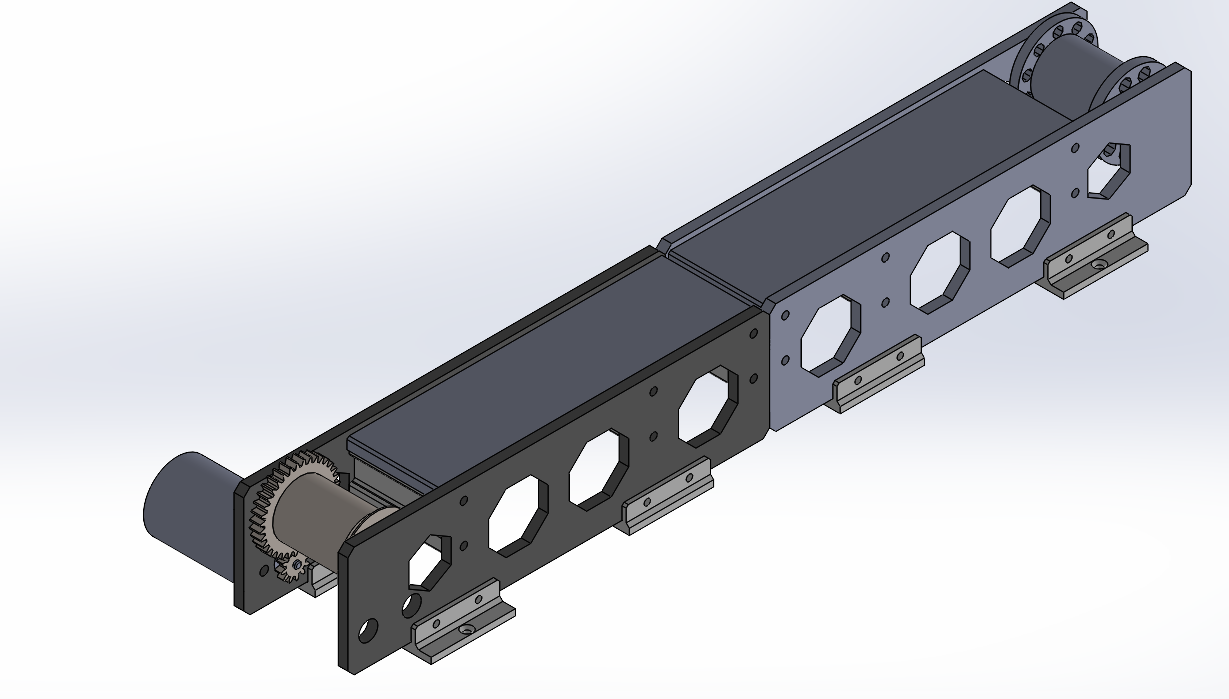
\includegraphics[width=0.75\textwidth]{Imagenes/Cinta.png} 
    \caption{Vista general de la cinta transportadora diseñada en CAD y fabricada mediante impresión 3D.}
    \label{fig:cinta_transportadora}
\end{figure}

\chapter{Resultados y Validación Cuantitativa}

\section{Evaluación y Cumplimiento de Objetivos}
En la Tabla~\ref{tab:cumplimiento_objetivos} se presenta la contrastación formal entre los objetivos específicos planteados al inicio del proyecto y el grado de concreción técnica alcanzado tras las modificaciones de hardware, firmware y software.

\begin{table}[H]
\centering
\small
\begin{tabular}{|p{3.8cm}|c|p{8.2cm}|}
\hline
\textbf{Objetivo Específico} & \textbf{Estado} & \textbf{Evidencia / Resultado Alcanzado} \\ \hline
1. Relevamiento y Diagnóstico & Cumplido & Identificación de fallas en transmisión por fricción, desacoples en I2C, modelo cinemático D-H inadecuado y saturación serial en ROS 2. \\ \hline
2. Definición de Módulos y Reingeniería & Cumplido & Rediseño de engranajes con chavetero, aislamiento SCL/SDA, migración de cinemática/trayectorias a STM32 y desarrollo de GUI en PyQt5. \\ \hline
3. Procesamiento Digital de Imágenes & Cumplido & Detección cenital a 30 FPS en espacio HSV, clasificación Cubo/Cono por Rect Ratio (87.2\% de efectividad global) y estimación de velocidad por compuertas espaciales. \\ \hline
4. Planificador Dinámico & Cumplido & Algoritmo de intercepción MRU en ROS 2 sincronizado con trayectoria quíntica local en STM32 ($T_{\text{traj}} = \max(T_{\text{MIN\_ROBOT}}, t_{\text{arribo}} - 0.15\text{ s})$). \\ \hline
5. Validación Experimental Cuantitativa & Cumplido & Tasa de éxito del 80.0\% (32/40) en ensayos dinámicos operativos válidos (74.4\% en el cómputo total de la celda 32/43) y 100\% en modo estático. \\ \hline
6. Supervisión Remota (Opcional) & No ejecutado & Descartado formalmente para priorizar la robustez del lazo de tiempo real de intercepción dinámica. \\ \hline
\end{tabular}
\caption{Matriz de cumplimiento de objetivos del Proyecto Final de Estudios.}
\label{tab:cumplimiento_objetivos}
\end{table}

\section{Metodología de Validación y Banco de Ensayos}
Para evaluar el desempeño global de la celda de manufactura, se definieron los casos de uso representativos de la operación industrial. Los ensayos se registraron audiovisualmente y se procesaron estadísticamente a partir de series de repeticiones continuas.

\section{Caso de Uso 1: Pick-and-Place Estático con Retroalimentación Visual}
\subsection{Descripción del Escenario}
Se dispuso el objeto en coordenadas cartesianas conocidas dentro del espacio de trabajo sobre la cinta detenida ($X = 215.0\text{ mm}$, $Z = 78.0\text{ mm}$, $Y \in [+10, +140]\text{ mm}$). Se realizaron 23 repeticiones evaluando el agarre magnético y la correcta clasificación hacia el depósito.

\subsection{Resultados Cuantitativos y Registro Experimental}
En la Tabla~\ref{tab:registro_estatico_manual} se detalla el registro empírico de las corridas experimentales correspondientes a la evaluación estática con retroalimentación visual ($N = 23$), consignando la coordenada longitudinal objetivo ($Y_{\text{pick}}$), el éxito en la fase de agarre (\textit{Pick}), la fase de depósito (\textit{Place}) y la clasificación morfológica obtenida.

\begin{table}[H]
\centering
\small
\begin{tabular}{|c|c|c|c|l|}
\hline
\textbf{N$^\circ$} & \textbf{$Y_{\text{pick}}$ [mm]} & \textbf{Pick} & \textbf{Place} & \textbf{Clasificación} \\ \hline
1  & 39.0  & $\checkmark$ & $\checkmark$ & Cubo \\ \hline
2  & 12.9  & $\checkmark$ & $\checkmark$ & Cono \\ \hline
3  & 92.2  & $\checkmark$ & $\checkmark$ & Cono \\ \hline
4  & 80.0  & $\checkmark$ & $\checkmark$ & Cubo \\ \hline
5  & 140.0 & $\checkmark$ & $\checkmark$ & Cubo \\ \hline
6  & 52.3  & $\checkmark$ & $\checkmark$ & Cono \\ \hline
7  & 118.5 & $\checkmark$ & $\checkmark$ & Cono \\ \hline
8  & 13.2  & $\checkmark$ & $\checkmark$ & Cubo \\ \hline
9  & 116.7 & $\checkmark$ & $\checkmark$ & Cubo \\ \hline
10 & 73.0  & $\checkmark$ & $\checkmark$ & Cubo \\ \hline
11 & 31.0  & $\checkmark$ & $\checkmark$ & Cono \\ \hline
12 & 113.0 & $\checkmark$ & $\checkmark$ & Cono \\ \hline
13 & 12.3  & $\checkmark$ & $\checkmark$ & Cono \\ \hline
14 & 91.5  & $\checkmark$ & $\checkmark$ & Cono \\ \hline
15 & 22.3  & $\checkmark$ & $\checkmark$ & Cubo \\ \hline
16 & 118.7 & $\checkmark$ & $\checkmark$ & Cubo \\ \hline
17 & 144.0 & $\checkmark$ & $\checkmark$ & Cono \\ \hline
18 & 10.0  & $\checkmark$ & $\checkmark$ & Cubo \\ \hline
19 & 23.7  & $\checkmark$ & $\checkmark$ & Cono \\ \hline
20 & 72.5  & $\checkmark$ & $\checkmark$ & Cono \\ \hline
21 & 75.2  & $\checkmark$ & $\checkmark$ & Cubo \\ \hline
22 & 129.3 & $\checkmark$ & $\checkmark$ & Cono \\ \hline
23 & 132.7 & $\checkmark$ & $\checkmark$ & Cubo \\ \hline
\end{tabular}
\caption{Registro experimental detallado de los ensayos de Pick-and-Place estático ($N = 23$).}
\label{tab:registro_estatico_manual}
\end{table}

\section{Caso de Uso 2: Intercepción Dinámica Síncrona a Velocidad Nominal}
\subsection{Descripción del Escenario y Registro Experimental}
Se realizaron un total de 35 ensayos continuos sobre la cinta transportadora en movimiento continuo, evaluando la sincronización temporal ($Y_{\text{pick}} = 120.0\text{ mm}$ con $T_{\text{anticipo}} = 0.15\text{ s}$), la toma mediante electroimán (\textit{Pick}), la elevación vertical pura ($Z_{\text{lift}} = 125.0\text{ mm}$) y el traslado/descarga en las cajas correspondientes según la geometría detectada (\textit{Place}).

En la Tabla~\ref{tab:registro_dinamico_completo} se detalla el registro empírico de todas las corridas experimentales, incluyendo la velocidad lineal observada ($V$), el resultado de las etapas de manipulación, la clasificación morfológica y las observaciones de campo.

\begin{table}[H]
\centering
\scriptsize
\begin{tabular}{|c|c|c|c|l|p{5.2cm}|}
\hline
\textbf{N$^\circ$} & \textbf{V [mm/s]} & \textbf{Pick} & \textbf{Objeto} & \textbf{Clasificación} & \textbf{Observaciones / Diagnóstico} \\ \hline
1  & 76.0  & $\checkmark$ & Cubo & Cubo & Operación exitosa \\ \hline
2  & 73.3  & $\times$     & Cono     & ---  & Fallo de agarre \\ \hline
3  & 79.3  & $\checkmark$ & Cubo & Cubo & Operación exitosa \\ \hline
4  & 76.1  & $\checkmark$ & Cono & Cono & Operación exitosa \\ \hline
5  & 83.9  & $\checkmark$ & Cono & Cono & Operación exitosa \\ \hline
6  & 31.9  & $\times$     & Cono     & ---  & Fallo en toma de velocidad \\ \hline
7  & 83.4  & $\checkmark$ & Cubo & Cubo & Operación exitosa \\ \hline
8  & 83.1  & $\checkmark$ & Cono & Cono & Operación exitosa \\ \hline
9  & 73.1  & $\checkmark$ & Cono & Cono & Operación exitosa \\ \hline
10 & 69.2  & $\checkmark$ & Cubo & Cubo & Operación exitosa \\ \hline
11 & 82.8  & $\checkmark$ & Cono & Cono & Operación exitosa \\ \hline
12 & 80.0  & $\checkmark$ & Cubo & Cubo & Operación exitosa \\ \hline
13 & 78.4  & $\checkmark$ & Cubo & Cubo & Operación exitosa \\ \hline
14 & 74.6  & $\checkmark$ & Cono & Cono & Operación exitosa \\ \hline
15 & 12.7  & $\times$     & Cubo     & ---  & Fallo en toma de velocidad \\ \hline
16 & 74.7  & $\times$     & Cono     & ---  & Fallo de agarre \\ \hline
17 & 74.0  & $\checkmark$ & Cubo & Cubo & Operación exitosa \\ \hline
18 & 86.1  & $\checkmark$ & Cono & Cono & Operación exitosa \\ \hline
19 & 74.7  & $\checkmark$ & Cubo & Cubo & Operación exitosa \\ \hline
20 & 88.9  & $\checkmark$ & Cono & Cono & Operación exitosa \\ \hline
21 & 35.9  & $\times$     & Cono     & ---  & Fallo en toma de velocidad \\ \hline
22 & 83.7  & $\times$     & Cubo     & ---  & Fallo de agarre \\ \hline
23 & 65.6  & $\checkmark$ & Cubo & Cubo & Operación exitosa \\ \hline
24 & 71.0  & $\checkmark$ & Cubo     & Cono & Error de clasificación: depósito en caja errónea \\ \hline
25 & 70.4  & $\checkmark$ & Cono & Cono & Operación exitosa \\ \hline
26 & 36.9  & $\times$     & Cono     & ---  & Fallo en toma de velocidad \\ \hline
27 & 70.1  & $\checkmark$ & Cubo & Cubo & Operación exitosa \\ \hline
28 & 76.4  & $\checkmark$ & Cubo & Cubo & Operación exitosa \\ \hline
29 & 76.3  & $\checkmark$ & Cono & Cono & Operación exitosa \\ \hline
30 & 70.4  & $\checkmark$ & Cubo & Cubo & Operación exitosa \\ \hline
31 & 82.7  & $\checkmark$ & Cono & Cono & Operación exitosa \\ \hline
32 & 70.9  & $\checkmark$ & Cubo & Cubo & Operación exitosa \\ \hline
33 & 67.1  & $\checkmark$ & Cono & Cono & Operación exitosa \\ \hline
34 & 66.7  & $\checkmark$ & Cubo & Cubo & Operación exitosa \\ \hline
35 & 70.4  & $\times$     & Cono    & ---  & Fallo de agarre \\ \hline
\end{tabular}
\caption{Registro experimental detallado de los ensayos de intercepción dinámica ($N = 35$).}
\label{tab:registro_dinamico_completo}
\end{table}

\subsection{Resultados Cuantitativos y Análisis Estadístico}
Del total de 35 registros de prueba:
\begin{itemize}
    
    \item Sobre los \textbf{35 ciclos operativos válidos}, el robot logró completar la maniobra de (\textit{Pick} exitoso) en \textbf{27 ocasiones}, representando una \textbf{tasa de éxito del 77.14\%}. Si se evalúa la totalidad de los 35 eventos incluyendo el desempeño físico de la cinta motriz, la tasa global de la celda se sitúa en el \textbf{91.4\%} ($32/35$).
    \item De los 27 casos donde se ejecutó un \textit{Pick} exitoso, en 1 ocasiones se registró un fallo de clasificacion (\textit{Place} $\times$), lo que representa un \textbf{3.7\%} de fallos en la clasificación morfológica.
    \item En los 8 casos donde fallo el (\textit{Pick} $\times$), representando una \textbf{tasa de error del 22.9\%}, se observó que 4 de ellos fueron consecuencia de una captura erronea de la velocidad, lo que representa un \textbf{11.4\%} de los casos, mientras que los 4 restantes se debieron a errores de agarre por fricción insuficiente, tambien un \textbf{11.4\%} de los casos.
    \item El rango de velocidad lineal registrado exitosamente osciló entre $66.5\text{ mm/s}$ y $88.9\text{ mm/s}$, con un promedio de $\bar{v} = 75.9\text{ mm/s}$.
\end{itemize}

En la Tabla~\ref{tab:resultados_dinamico} se presenta el desglose consolidado de los modos de fallo observados durante las pruebas dinámicas.

\begin{table}[H]
\centering
\begin{tabular}{lcc}
\toprule
\textbf{Resultado de la Operación} & \textbf{Eventos} & \textbf{Porcentaje (\%)} \\
\midrule
\textit{Pick} + \textit{Place} clasificado correcto & 26 & 74.3\% \\
\textit{Pick} exitoso & 27 & 77.1\% \\
Fallo en clasificación morfológica & 1/27(\textit{Pick}) exitosos, & 3.7\% \\
Fallo en agarre / sincronismo inicial (\textit{Pick} $\times$) & 4 &11.4\% \\
Fallo en captura de velocidad (\textit{Pick} $\times$) & 4 &11.4\% \\
\midrule
\textbf{Total de Ensayos Operativos Válidos} & \textbf{35} & \textbf{100.0\%} \\
\bottomrule
\end{tabular}
\caption{Rendimiento cuantitativo y análisis de fallos en modo dinámico continuo ($N = 35$).}
\label{tab:resultados_dinamico}
\end{table}

\section{Evaluación de Límites Operativos: Variación Dinámica de Velocidad}
Para determinar la ventana de operación real de la celda de manufactura y validar la robustez del algoritmo de factibilidad cinemática, se diseñó un ensayo específico variando la velocidad de la cinta transportadora en tiempo real mediante la regulación analógica del potenciómetro en su motor de tracción.

\textbf{Límite Inferior de Operación ($67\text{ mm/s}$):} 
Se determinó empíricamente que la velocidad mínima viable para la ejecución del ciclo continuo es de aproximadamente $67\text{ mm/s}$. Por debajo de este umbral, el motor de corriente continua (DC) encargado de la tracción carece del torque electromagnético necesario para vencer la fricción mecánica del sistema de rodillos y bujes. Esto provoca que la banda se detenga o avance de forma irregular (a tirones), invalidando la premisa de Movimiento Rectilíneo Uniforme (MRU) requerida por el algoritmo de visión para predecir con exactitud el instante de intercepción.

\textbf{Límite Superior y Cota Máxima Exitosa ($108.9\text{ mm/s}$):}
Al incrementar la velocidad de la banda progresivamente, se logró registrar de manera exitosa (y documentar en el registro audiovisual) intercepciones dinámicas hasta una velocidad máxima de $108.9\text{ mm/s}$. En estas condiciones, la reducción del tiempo de recorrido de la pieza pone a prueba tanto la frecuencia de actualización del nodo de visión como la respuesta dinámica del manipulador, logrando concretar la maniobra sin pérdida de pasos ni desprendimiento magnético.

\textbf{Restricción Cinemática y Aborto Preventivo ($> 108.9\text{ mm/s}$):}
Al forzar la cinta por encima de la celeridad máxima comprobada, el sistema exhibe el comportamiento de seguridad diseñado en el nivel de supervisión (máquina de estados). Cuando el orquestador evalúa la nueva velocidad entrante, el cálculo analítico determina que el tiempo restante para que la pieza alcance el punto nominal de recolección ($t_{disp}$) es estrictamente inferior al tiempo mínimo físico demandado por los motores para ejecutar la curva quíntica de aproximación ($T_{\text{MIN\_ROBOT}}$). 

Al detectarse esta condición ($t_{disp} < T_{\text{MIN\_ROBOT}}$), el algoritmo clasifica la intercepción como cinemáticamente \textbf{No Factible}. En lugar de intentar un seguimiento reactivo ciego que desencadenaría vibraciones severas o un desfasaje espacial, el controlador asume una postura conservadora: el manipulador se mantiene completamente inmóvil en su posición de guardia dejando pasar la pieza, mientras la interfaz gráfica (GUI) notifica al operador que el ciclo fue abortado por exceso de velocidad en la banda. Este comportamiento valida la seguridad integral de la celda, protegiendo los actuadores y previniendo colisiones.

\section{Registro Audiovisual y Demostraciones}
Para facilitar la evaluación externa y la verificación experimental de los resultados obtenidos, los registros audiovisuales de los ensayos se encuentran disponibles en el repositorio multimedia institucional del proyecto:
\begin{itemize}
    \item \textbf{Video Anexo 1 (Pick-and-Place Estático):} \href{https://universidadcuyo-my.sharepoint.com/:v:/g/personal/molina_matias_uncuyo_edu_ar/IQAEfuTCPxe3T4dsjXcwBnaGAX35Iyutr4qPirEA1u29M0E?e=xh17bC&nav=eyJyZWZlcnJhbEluZm8iOnsicmVmZXJyYWxBcHAiOiJTdHJlYW1XZWJBcHAiLCJyZWZlcnJhbE1vZGUiOiJtaXMiLCJyZWZlcnJhbFZpZXciOiJwb3N0cm9sbC1jb3B5bGluayIsInJlZmVycmFsUGxheWJhY2tTZXNzaW9uSWQiOiIwYjc5ZTc4OC1jYmUwLTQ1OWYtOTJlZi04ZTNkYzM1Yjc1MjcifX0%3D}{Acceso al registro audiovisual del Caso 1 (SharePoint / OneDrive UNCUYO)}, exhibiendo la calibración óptica, repetibilidad y validación del lazo cerrado de visión.
    \item \textbf{Video Anexo 2 (Intercepción Dinámica Continua V2):} \href{https://universidadcuyo-my.sharepoint.com/personal/molina_matias_uncuyo_edu_ar/_layouts/15/stream.aspx?id=%2Fpersonal%2Fmolina%5Fmatias%5Funcuyo%5Fedu%5Far%2FDocuments%2FPFE%2FCaso%202%20Dinamico%20Continuo%2FCasoDinamico2%2Emkv&referrer=StreamWebApp%2EWeb&referrerScenario=AddressBarCopied%2Eview%2Ec2cd7f54%2D5756%2D4111%2Dabd3%2D65ea02b11d6f}{Acceso al registro audiovisual del Caso 2 (SharePoint / OneDrive UNCUYO)}, exhibiendo la detección en compuertas espaciales, sincronización temporal MRU, intercepción en movimiento, elevación vertical pura ($Z_{\text{lift}}$) y descarga clasificada.
    \item \textbf{Video Anexo 3 (Failsafe y Retorno Rápido):} \href{https://universidadcuyo-my.sharepoint.com/:v:/g/personal/molina_matias_uncuyo_edu_ar/IQC4HhHrg-AMSam3l6sVpuQnAaCE1OA0pd9p2rAQQmxLEsE?e=YsTjAv&nav=eyJyZWZlcnJhbEluZm8iOnsicmVmZXJyYWxBcHAiOiJTdHJlYW1XZWJBcHAiLCJyZWZlcnJhbE1vZGUiOiJtaXMiLCJyZWZlcnJhbFZpZXciOiJwb3N0cm9sbC1jb3B5bGluayIsInJlZmVycmFsUGxheWJhY2tTZXNzaW9uSWQiOiIzNzNjZGEwNS04NGYwLTQ2MTYtYTJjNi1kNDBiYjBlMGJkYjkifX0%3D}{Acceso al registro audiovisual del Caso 3 (SharePoint / OneDrive UNCUYO)}: validación del comportamiento de la máquina de estados ante desprendimiento de pieza y rechazo cinemático por exceso de velocidad.
    \item \textbf{Video Anexo 4 (Variación Dinámica de Velocidad):} \href{https://universidadcuyo-my.sharepoint.com/personal/molina_matias_uncuyo_edu_ar/_layouts/15/stream.aspx?id=%2Fpersonal%2Fmolina%5Fmatias%5Funcuyo%5Fedu%5Far%2FDocuments%2FPFE%2FVariacion%20de%20Velocidad%2FVariacionVelocidad%2Emkv&referrer=StreamWebApp%2EWeb&referrerScenario=AddressBarCopied%2Eview%2Ed1eaa3d8%2D2e32%2D4f63%2D8ca6%2D296c463a265b}{Acceso al registro audiovisual del Caso 4 (SharePoint / OneDrive UNCUYO)}: exhibición de la ventana de operación real de la celda, incluyendo límites inferior y superior de velocidad, así como el comportamiento de rechazo cinemático ante exceso de velocidad.
\end{itemize}

\chapter{Conclusiones, Limitaciones y Trabajos Futuros}

\section{Conclusiones}
En el presente Proyecto Final de Estudios se transformó una plataforma experimental estática en una celda de manufactura robotizada orientada a la manipulación dinámica continua. Las principales conclusiones técnicas son:
\begin{enumerate}
    \item \textbf{Arquitectura Embebida y Regularidad Temporal:} La migración de la cinemática inversa analítica y de la generación de trayectorias quínticas ($C^2$) hacia la FPU del microcontrolador STM32F446RE redujo sustancialmente el tráfico sobre el canal de comunicaciones en ROS 2, favoreciendo perfiles de velocidad suaves a 100 Hz.
    \item \textbf{Percepción Visual y Clasificación:} La estimación de velocidad lineal mediante compuertas espaciales fijas en OpenCV desacopló el cálculo temporal de la latencia de renderizado de la UI. Asimismo, el enfoque combinado de \textit{Extent} y \textit{Rect Ratio} ofreció una discriminación geométrica invariante a la orientación con un 87.2\% de efectividad global en las pruebas realizadas.
    \item \textbf{Reingeniería Mecánica y Eléctrica:} La incorporación de uniones por chaveta en los ejes de los motores paso a paso y la reorganización del cableado I2C resolvieron satisfactoriamente las fallas críticas de deslizamiento torsional e interferencia electromagnética observadas en el prototipo original.
\end{enumerate}

\section{Limitaciones del Sistema}
Se identifican las siguientes limitaciones en el prototipo actual:
\begin{itemize}
    \item \textbf{Rigidez Mecánica y Carga Útil:} La estructura fabricada en impresión 3D (PLA/PETG) presenta flexiones elásticas marginales ante aceleraciones bruscas, limitando la carga útil del efector a piezas livianas ($< 80\text{ g}$).
    \item \textbf{Efector Magnético:} El sistema de sujeción restringe la manipulación a objetos con propiedades o insertos ferromagnéticos y resulta sensible a desalineaciones angulares en la superficie de contacto.
    \item \textbf{Dinámica de Tracción de la Banda:} La cinta transportadora tiende a frenarse ocasionalmente debido a la fricción acumulada en los apoyos mecánicos y desalineaciones de tensión, lo que introduce variaciones momentáneas en el perfil de velocidad de transporte de las piezas.
    \item \textbf{Sensibilidad a la Iluminación:} Si bien la calibración interactiva HSV es rápida, variaciones drásticas en la luz solar ambiental pueden exigir reajustes periódicos de los umbrales cromáticos.
\end{itemize}

\section{Trabajos Futuros}
\begin{itemize}
    \item Desarrollar un efector final por succión neumática (ventosa de vacío) para ampliar el abanico de materiales manipulables.
    \item Rediseñar los materiales de la cinta transportadora y rodillos de tracción, reemplazando la cinta antideslizante tipo lija para pisos utilizada actualmente en los cilindros por bandas de caucho vulcanizado o recubrimientos de poliuretano industrial con textura de alto agarre, optimizando el coeficiente de fricción para evitar caídas y deslizamientos sin comprometer la fluidez del movimiento.
    \item Desarrollar e integrar un gemelo digital (\textit{Digital Twin}) en entornos de simulación robótica (como Gazebo o Isaac Sim) sincronizado en tiempo real con la telemetría micro-ROS, permitiendo la validación previa de trayectorias complejas, prevención de colisiones y pruebas virtuales de nuevas secuencias operativas.
    \item Implementar el módulo de supervisión remota e IoT (planteado inicialmente como objetivo opcional), integrando el microcontrolador ESP32 para la transmisión inalámbrica de telemetría, alertas operativas y monitoreo de estados en tiempo real a través de un panel de control interactivo en Node-RED.
    \item Incorporar un sistema de iluminación LED difusa controlada para aislar completamente la celda de las condiciones de luz externa.
\end{itemize}

\section{Guía de Reproducibilidad y Entorno Técnico}
Para facilitar la reproducción del desarrollo por parte de futuros grupos de trabajo, se detallan las especificaciones técnicas del entorno y los recursos necesarios:
\begin{itemize}
    \item \textbf{Sistema Operativo de Alto Nivel:} Ubuntu 22.04 LTS con ROS 2 Humble Hawksbill.
    \item \textbf{Librerías Principales:} Python 3.10, OpenCV 4.8, PyQt5, NumPy.
    \item \textbf{Entorno de Firmware:} STM32CubeIDE v1.14+, FreeRTOS v10.3, micro-ROS for STM32 (UART2 con DMA a 115200 baudios).
    \item \textbf{Hardware Principal:} Placa STM32 Nucleo-F446RE, Drivers A4988 (configurados a 1/8 de micropaso), Encoders magnéticos AS5600 (I2C a 400 kHz), Multiplexor TCA9548A, Cámara web HD 720p a 30 FPS.
    \item \textbf{Fabricación y Código Fuente:} El ensamblaje final de la maqueta en SolidWorks, junto con la totalidad del código fuente del supervisor en ROS 2 y el firmware del microcontrolador, se encuentran de acceso público en el repositorio de GitHub del autor: \url{https://github.com/bexemat/PFE-Molina-Matias}.
\end{itemize}

\section{Declaración sobre el Uso de Inteligencia Artificial}
En el marco del presente Proyecto Final de Estudios, se utilizó activamente el modelo de lenguaje de Inteligencia Artificial \textbf{Gemini Pro} (al cual se tuvo acceso mediante una suscripción profesional gratuita para estudiantes por el plazo de un año) operando como asistente técnico y de programación.

Durante la etapa inicial de relevamiento y diagnóstico, esta herramienta resultó de fundamental ayuda para analizar el código heredado. Su capacidad de procesamiento de texto estructurado permitió construir mapas conceptuales para comprender el funcionamiento de la estructura monolítica existente, facilitando la toma de decisiones estratégicas sobre cómo modularizar el firmware y dictaminar con precisión qué segmentos lógicos del sistema original era conveniente conservar y cuáles debían ser descartados o reescritos por completo.

Posteriormente, el aporte más significativo se centró en la creación y estructuración de la Interfaz Gráfica de Usuario (GUI). Dado que no se contaba con conocimientos previos en el framework \textbf{PyQt5}, la inteligencia artificial permitió desarrollar por completo la compleja integración entre la interfaz visual y la arquitectura de comunicaciones de \textbf{ROS 2}. Su asistencia en este apartado fue fundamental para lograr un puente de comunicación estable, un renderizado fluido y el correcto mapeo de eventos.

Para el resto del desarrollo del firmware embebido y los nodos analíticos, la inteligencia artificial se empleó bajo una metodología estrictamente estructurada. En lugar de delegar la generación de código monolítico, el flujo de trabajo consistió en diagramar las arquitecturas conceptuales, diseñar funciones modulares reducidas a su mínima expresión y dictaminar de manera precisa las entradas y salidas requeridas para cada bloque lógico. Este enfoque metodológico permitió acelerar los tiempos de codificación y depuración, manteniendo en todo momento el control absoluto sobre el determinismo, la seguridad y la arquitectura global del sistema.

Adicionalmente, en lo que respecta a la confección del presente informe técnico, la herramienta resultó ser un recurso sumamente valioso para la generación automatizada del código \LaTeX{} empleado en el diseño y renderizado de los diversos esquemas, flujogramas y diagramas de bloques (mediante el uso del paquete Ti\textit{k}Z) que ilustran la arquitectura conceptual y funcional de la celda robótica.
\nocite{*}
\bibliographystyle{ieeetr}
\bibliography{referencias}

\end{document}